\documentclass[a4paper, 10pt]{article}
\usepackage[utf8]{inputenc}
\usepackage[czech, british]{babel}
\usepackage[autostyle]{csquotes}
\usepackage{multicol}
\usepackage[top=1.5cm, left=2cm, right=1cm, bottom=2cm]{geometry}
\usepackage{tikz}
\usepackage{eso-pic}
\usepackage[T1]{fontenc}
\usepackage{setspace}
\usepackage{dashrule}
\usepackage{amssymb}
\usepackage{anyfontsize}
%poslední balík
\usepackage[pdftex]{hyperref}
\hypersetup{colorlinks=true, linkcolor=gray}
 
%příkazy pro hypertextové odkazy
\newcommand{\hylo}[2]{\hyperlink{#1}{#2}}
\newcommand{\hyl}[2]{\vspace{-15pt}\hspace{28pt}\hyperlink{#1}{\textbf{$\rightarrow$#2}}}
\newcommand{\hyt}[1]{\hypertarget{#1}{}}


\def\everypar{\parindent=-10mm} %předsazení prvního řádku odstavce
\newcommand{\chord}[2][l]{\makebox[0pt][#1]{\textbf{\begin{tabular}[b]{@{}l@{}}#2\\
				\mbox{}\end{tabular}}}} %příkaz pro akordy
\pdfminorversion=7		

%%KONVENCE
	% charakteristiky akordů kromě moll se píšou do horního indexu
	% pochody v basu se píšou do dolního indexu (\bas)
%AKORDY
\newcommand{\bas}[1]{/\textsubscript{#1}}%dolní index pro přechody v basu
\newcommand{\add}[1]{\textsuperscript{#1}}%manuální horní index
\newcommand{\maj}{\textsuperscript{$\triangle$}}%maj7 akordy
\newcommand{\sus}[1]{\textsuperscript{sus#1}}%sus[] akordy
\newcommand{\dm}{\textsuperscript{\Large{$\circ$}}}%dim akordy (zmenšený septakord c-es-ges-a, diminished)
\newcommand{\hdm}{\textsuperscript{\large{$\varnothing$}}}%m7/5- akordy (malý zmenšený septakord c-es-ges-b, half diminished)
\newcommand{\+}{\textsuperscript{+}}%aug akordy (C-E-G#)
\newcommand{\bb}{\textsuperscript{\Large$\flat$}}%béčko
\newcommand{\kk}{\textsuperscript{\#}}%křížek
\newcommand{\2}{\textsuperscript{2}}%2
\newcommand{\4}{\textsuperscript{4}}%4
\newcommand{\5}{\textsuperscript{5}}%5
\newcommand{\6}{\textsuperscript{6}}%6
\newcommand{\7}{\textsuperscript{7}}%7
\newcommand{\9}{\textsuperscript{9}}%9
\newcommand{\note}[1]{\emph{#1}\vspace{-20pt}}

%MEZERY
%horizontální
\newcommand{\bc}{\hspace{60pt}}%velký akord navíc
\newcommand{\nc}{\hspace{30pt}}%akordy navíc
\newcommand{\sm}{\hspace{7pt}}%extra mezera malá
\newcommand{\mm}{\hspace{15pt}}%extra mezera střední
\newcommand{\nv}{\hspace{28pt}}%no verse - odsazení prvního řádku pro neoznačené texty
%vertikální
\newcommand{\vnv}{\vspace{25pt}}%vertical no verse - svislé odsazení
\newcommand{\vinv}{\vspace{-2mm}\\}%vertical in verse - svislé odsazení
\newcommand{\ns}{\vspace{-20pt}}%no space - zrušení mezery mezi slokami
\newcommand{\cns}{\vspace{-35pt}}%no space - zrušení mezery mezi slokami
\newcommand{\lsp}[1]{\vspace{-13pt}\hspace{25pt}\hdashrule{#1cm}{1pt}{3pt}\vspace{-23pt}}%oddělení slok linkou

%MAIN
\newcommand{\song}[1]{\section*{\Huge\sc\hypersetup{linkcolor=black}\hyperlink{obsah}{\textbf{#1}}\hypersetup{linkcolor=gray}\Large\hyperlink{obsah}{\hspace{2mm} $\rightarrow$~obsah}}
}%název
\newcommand{\sub}[1]{\vspace{-10mm}\subsection*{\large\expandafter\sc{#1}}}%podnázev
\newcommand{\refrain}[1]{\vspace{20pt}\textbf{{R:}}\hspace{0.5em}{#1}}%refrain
\newcommand{\refrainn}[2]{\vspace{20pt}\textbf{{R{#1}:}}\hspace{-0.1em}{#2}}%číslovaný refrain
\newcommand{\refsm}[1]{\textbf{R{#1}.}}%malý refrain
\newcommand{\refsme}[1]{\vspace{20pt}\textbf{R{#1}.}}%malý refrain oddělený od sloky
\newcommand{\intro}[1]{\vspace{20pt}\textbf{I:}\hspace{0.9em}{#1}}%intro
\newcommand{\bridge}[1]{\vspace{20pt}\textbf{B:}\hspace{0.6em}{#1}}%bridge
\newcommand{\solo}[1]{\vspace{20pt}\textbf{S:}\hspace{1.2em}{#1}}%solo
\newcommand{\solon}[2]{\vspace{20pt}\textbf{S{#1}:}\hspace{1.2em}{#2}}%solo
\newcommand{\solosm}[1]{\vspace{20pt}\textbf{S{#1}.}\hspace{1.2em}}%solo
\newcommand{\cod}[1]{\vspace{20pt}\textbf{C:}\hspace{0.6em}{#1}}%coda
\newcommand{\vers}[2]{\vspace{20pt}\textbf{#1.}\hspace{0.7em}{#2}}%sloka
\newcommand{\rep}[1]{$\backslash$: {#1} :$\backslash$}%repetice
\newcommand{\rec}[1]{\textit{rec: }{/#1/}}%recitativ

\newcommand{\placepic}[4]{\AddToShipoutPictureFG*{\put(\LenToUnit{#1\paperwidth},\LenToUnit{#2\paperheight}){\vtop{{\null}\includegraphics[width=#3pt]{#4}}}}}

\newcommand{\placetextbox}[3]{\AddToShipoutPictureFG*{\put(\LenToUnit{#1\paperwidth},\LenToUnit{#2\paperheight}){\vtop{{\null}\begin{minipage}{\linewidth}{\fontfamily{cmtt}\selectfont\begin{large}\parbox{\linewidth}{\hspace{22pt}#3}\end{large}}\end{minipage}}}}}

\newcommand{\interpret}[2]{\AddToShipoutPictureFG*{\put(\LenToUnit{0.9\paperwidth},\LenToUnit{0.98\paperheight}){\vtop{{\null}\begin{minipage}{\linewidth}{\parbox{\linewidth}{\hyperlink{#1}{$\rightarrow$~#2}}}\end{minipage}}}}}

\newcommand{\interpretdva}[2]{\AddToShipoutPictureFG*{\put(\LenToUnit{0.7\paperwidth},\LenToUnit{0.98\paperheight}){\vtop{{\null}\begin{minipage}{\linewidth}{\parbox{\linewidth}{\hyperlink{#1}{$\rightarrow$~#2}}}\end{minipage}}}}}

\author{František Hluchník}

\begin{document}
\pagestyle{empty}
\newgeometry{bottom=10mm, right=10mm}
%obrázek na pozadí
\tikz[remember picture,overlay] \node[opacity=1,inner sep=0pt] at (current page.center){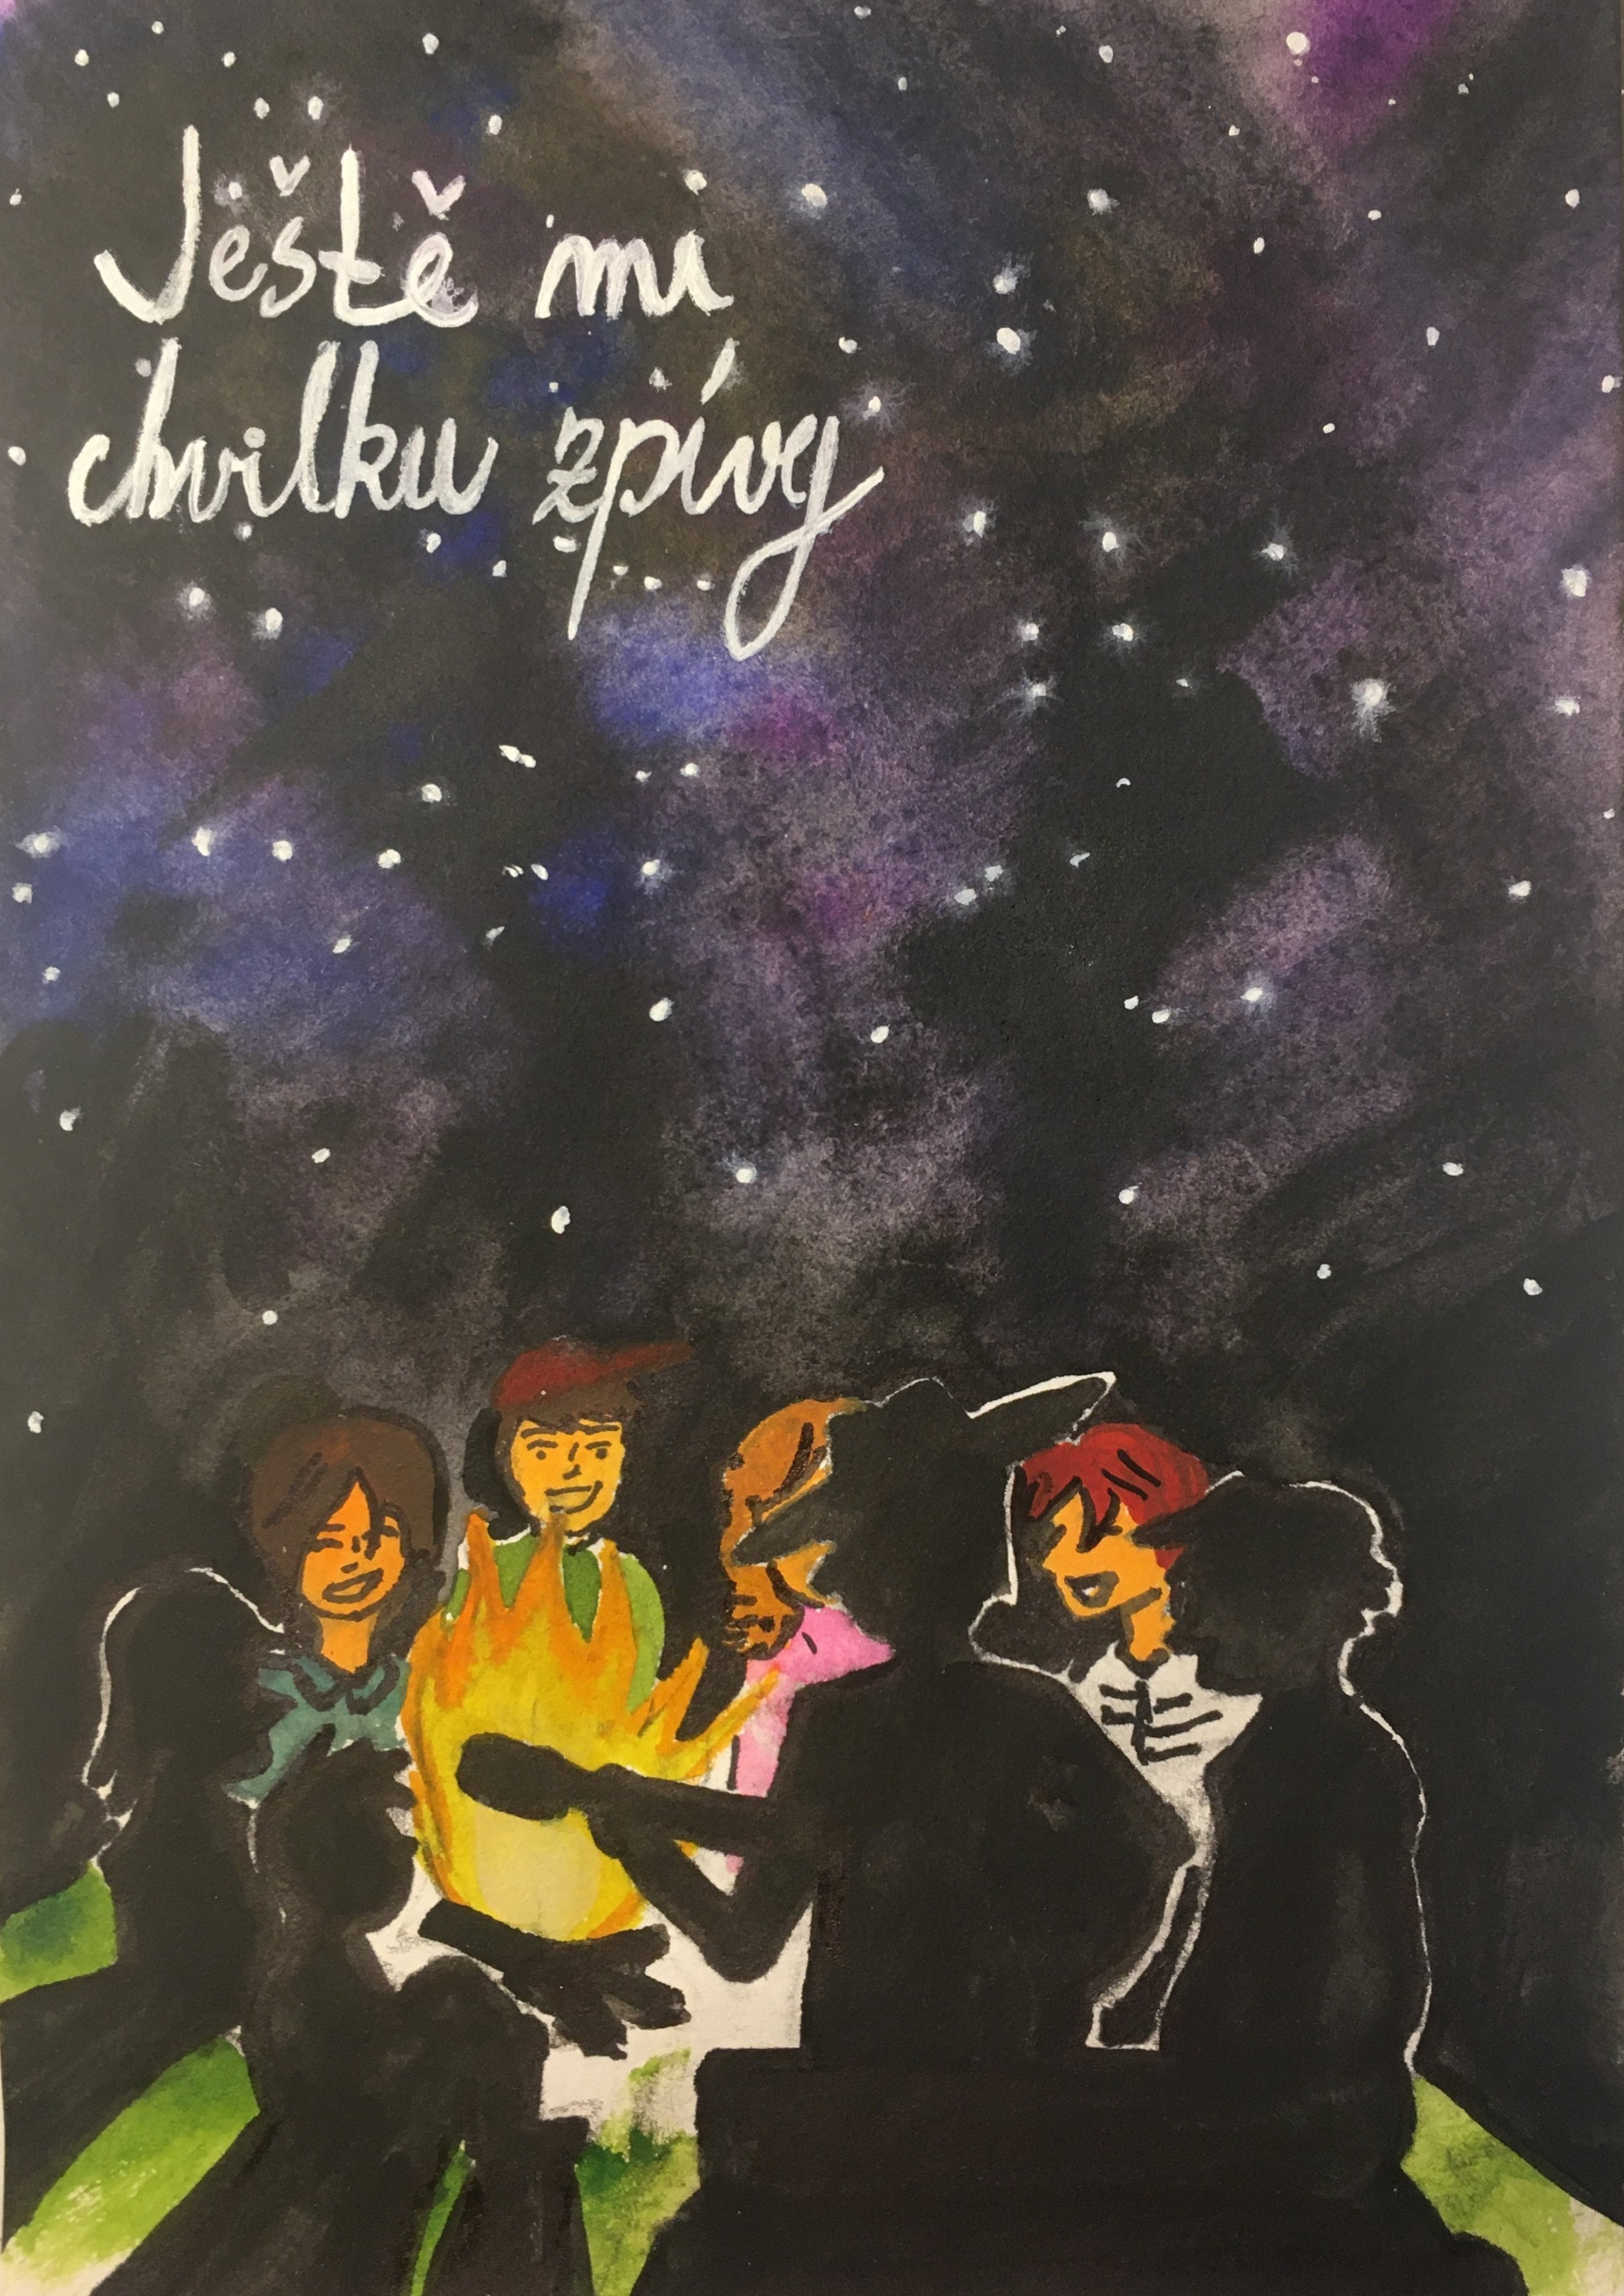
\includegraphics[width=\paperwidth,height=\paperheight]{obrazky/titpic.jpg}};
\placetextbox{0.18}{0.715}{
		\fontfamily{frc}
		\selectfont
		\color{white}
		\fontsize{35}{40}
		\textbf{\textbf{\textit{lidové písničky}}}
}
\restoregeometry
\newpage
\clearpage\mbox{}\clearpage
\vspace*{5cm}
\begin{center}
\begin{LARGE}
	Ještě mi chvilku zpívej
\end{LARGE}

\begin{large}
	výběr
	
	lidové písničky
\end{large}
\vspace{1cm}
\end{center}
\newpage
\vspace*{\fill}
%\hspace{10mm}sepsal František Hluchník\\
\hspace{10mm}obálku nakreslila Ivana Vlčková\\
\begin{otherlanguage}{czech}
Brno, \today\\
\end{otherlanguage}
%až se bude tisknout:
1. tištěné vydání\\
verze 1.76, odvozeno z verze 7.11 \textit{Ještě mi chvilku zpívej}\\
vysázeno jazykem \LaTeXe
\vspace{2cm}
\newpage
\vspace*{5cm}
\begin{center}
\begin{Huge}
	\fontfamily{frc}
	\selectfont
	Ještě mi chvilku zpívej
\end{Huge}
%\vspace{1cm}

\begin{large}
	výběr
	
	lidové písničky
\end{large}
\vspace{1cm}

\begin{Large}
František Hluchník
\vspace{4mm}

2020
\end{Large}
\end{center}
\newpage

\clearpage
\setcounter{page}{5}
\pagestyle{plain}

\begin{Large}
\hyt{ajatakadzivocka}
\song{A ja taka dzivočka}

\vers{1}{
\chord{Em}A ja \chord{Am}taka \chord{H\7}dzivo\chord{Em}čka, \chord{H\7}cingilingi \chord{Em}bom.\\
\chord{Em}Rada \chord{Am}vijem \chord{H\7}pire\chord{Em}čka, \chord{H\7}cingilingi \chord{Em}bom.\\
\rep{\chord{G}Rada vijem, \chord{D}rada \chord{G}dam, \chord{C}cingilingi \chord{Am}bom, bom, \chord{H\7}bom,\\
\chord{Em}i za \chord{Am}kalap \chord{H\7}zakla\chord{Em}dam, \chord{H\7}cingilingi \chord{Em}bom.}
}

\vers{2}{
A ja taka jak i mac, cingilingi bom.\\
Čarne oči mušim mac, cingilingi bom.\\
\rep{Čarne oči mac mala, cingilingi bom, bom, bom,\\
ja še na ňu podala, cingilingi bom.}
}

\vers{3}{
A ty, cigan, dobre hraj, cingilingi bom.\\
Na dzivčata něžmurkaj, cingilingi bom.\\
\rep{Na dzivčata na šumne, cingilingi bom, bom, bom,\\
naj něchodza po humně, cingilingi bom.}
}
\newpage

\hyt{anickadusickanekasli}
\song{Anička, dušička, nekašli}

\vers{1}{
\rep{\chord{G}Kdo si tu \chord{D}pěsničku \chord{G}zazpí\chord{G\7}vá? \chord{C}Veselá \chord{D}partyja z \chord{G}Mistřína.}\\
\rep{\chord{G}Oni si ju prevelice \chord{C}zpěva\chord{Am}jú, \sm\chord{D}keď sa večer za děvčaty \chord{G}trajda\chord{Em}jú.\\
\chord{G}Trajdajú, \chord{D}zpěvajú \chord{G}veli\chord{G\7}ce, \chord{C}dyž idú \chord{D}pres pole \chord{G}k muzice.}
}

\vers{2}{
\rep{Anička, dušička, nekašli, aby ma pri tebja nenašli.}\\
\rep{Já ťa chytím polúbím aj postískám, a pritom si prevelice zavýskám,\\
zavýskám na celú dědinu, jakú mám šikovnú děvčinu.}
}

\vers{3}{
\rep{Z Mistřína chlapci sa scházajú, nikemu pobit sa nedajú.}\\
\rep{Jak ho chytnú, tak ho bijú vesele, po paprčách po papuli, po čele,\\
potom sa šikovno ztrácajú, pres pole domů sa vracajú.}
}

\vers{4}{
\rep{Močila konopu, močila, žaba jej pod sukňu skočila.}\\
\rep{Aj ty, žabka, žabulenka vyskoč ven, lebo ťa dám vyšikovat žandárem,\\
močila konopu, močila, žaba jej pod sukňu skočila.}
}
\newpage

\hyt{beskydebeskyde}
\song{Beskyde, Beskyde}

\vers{1}{
\chord{E}Beskyde, Besky\chord{H\7}de, kdo po tobě i\chord{E}de?\\
\rep{\chord{A}Černooký bača \chord{E}ovečky \chord{H\7}zatá\chord{E}čá.}
}

\vers{2}{
Aj, bačo, bačo náš, černú košulku máš.\\
\rep{Kdo ti ju vypere, když maměnky nemáš?}
}

\vers{3}{
Já nemám maměnku, ale mám galánku.\\
\rep{Ona mi vypere černú košulenku.}
}

\vers{4}{
Ona ju vypere a pěkně vyválí,\\
\rep{až půjdu k muzice, každý ňa pochválí.}
}

\vers{5}{
Všeci sa starajú o moju chudobu\\
\rep{a já sa nestarám, chvála Pánu Bohu.}
}

\vers{6}{
Všeci sa ženíja, vojny sa bojíja\\
\rep{a já sa nežením, vojny sa nebojím.}
}
\newpage

\hyt{breclavskakasarna}
\song{Břeclavská kasárňa}

\vers{1}{
\chord{C}Břeclavská kasárňa \chord{G}malova\chord{C}ná,\\
\chord{C}malujú ju chlapci \chord{G}se šavla\chord{C}ma.\\
\rep{\chord{G}Chlapci se šavlama, \chord{C}děv\chord{G}ča\chord{C}ta \chord{F}sl\chord{C}za\chord{G}ma,\\
\chord{C}Břeclavská kasárňa \chord{G}malova\chord{C}ná.}
}

\vers{2}{
Břeclavská kasárňa široký dvůr,\\
po něm sa procházá šohajek můj.\\
\rep{Po něm sa procházá, převelice pláče,\\
až sa ta kasárňa celá třase.}
}

\vers{3}{
Dočkajte děvčata tři měsíce,\\
bude nás rukovat na tisíce.\\
\rep{Vy budete plakat, my budeme skákat\\
v Břeclavskej hospodě při muzice.}
}
\newpage

\hyt{cojstehasici}
\song{Co jste, hasiči}

\vers{1}{
\chord{G}Co jste, \chord{C}hasi\chord{G}či, co jste děla\chord{D}li?\\
\rep{\chord{D}Že jste nám ten pivo, pivo, pivovárek shořet \chord{D\7}necha\chord{G}li.}
}

\vers{2}{
Shořet nechali i tu hospodu.\\
\rep{My, staří mazáci, staří ulejváci, máme pít vodu!}
}

\vers{3}{
Vodu nepijem, my pijeme rum.\\
\rep{Voda je pro žáby, víno je pro báby, my pijeme rum.}
}

\vers{4}{
Vodu nepijem, my pijeme rum.\\
\rep{My pívečko pijem, vesele si žijem, za pár jdem domů.}
}

\vers{5}{
Za pár, za čtyři, už tu nebudem,\\
\rep{už vás milí páni, páni lampasáci, zdravit nebudem.}
}
\newpage

\hyt{cosatosupoce}
\song{Co sa to šupoce}

\vers{1}{
\rep{\chord{G}Co sa to šu\chord{D}poce \chord{D\7}za tú stodo\chord{G}lú?}\\
\rep{\chord{C}Šohajovi koně, \chord{G}šohajovi koně, šohajovi \chord{D}koně \chord{D\7}vody nema\chord{G}jú}
}

\vers{2}{
\rep{Nemajú, nemajú, chcelo sa jim pit.}\\
\rep{Mosela šenkéřka pro vínečko jít.}
}

\vers{3}{
\rep{Špatný si synečku, špatný hospodář,}\\
\rep{že svojim koníčkom vody nepodáš.}
}

\vers{4}{
\rep{Špatná si dcerečko, špatná kuchařka,}\\
\rep{že sa ti na plotně pálí zásmažka.}
}

\vers{5}{
\rep{Špatná si dcerečko, špatná hospodyň,}\\
\rep{že sa ti na plotně pálí petrolín.}
}

\vers{6}{
\rep{Špatná si dcerečko, špatná švadlena,}\\
\rep{žes ušila trenky až po kolena.}
}

\vers{7}{
\rep{Neošidil som sa, iba na ženě.}\\
\rep{Koňa možeš prodat, vola vyhandlovat, vola vyhandlovat, ale ženu nie.}
}
\newpage

\hyt{ceresnicky}
\song{Čerešničky}

\vers{1}{
\chord{C}Čerešničky, čerešničky, če\chord{F}reš\chord{C}ně,\\
\chord{C}vy ste sa ně \chord{A}rozsypaly \chord{Dm} na\sm \chord{C}ces\chord{G}tě.\\
\rep{\chord{D}Kdo vás najde \chord{D\7}ten vás posbí\chord{G}rá,\\
\chord{G\7}já som mala \chord{C}včera \chord{G\7}večer frají\chord{C}ra.}
}

\vers{2}{
Bol to frajír malovaný jak růža,\\
toho bych si vyvolila za muža.\\
\rep{Ani bych mu robit nedala,\\
jenom jako růžu bych ho chovala.}
}

\vers{3}{
Ako růžu, ako růžu červenú,\\
já bych bola jeho ženú milenú,\\
\rep{já bych bola jeho lilija\\
a on moja růža, růža červená.}
}

\vers{4}{
A keď bych ho, a keď bych ho dostala,\\
pak bych se mu, pak bych se mu vysmála.\\
\rep{Robit bude a já tancovat,\\
preca já si umím chlapa vychovat.}
}
\newpage

\hyt{cerneocijdetespat}
\song{Černé oči, jděte spát}

\vers{1}{
\chord{D}Černé oči, jdě\chord{A}te \chord{D}spát. \chord{D}Černé \chord{D\7}oči \chord{G}jdě\chord{H\7}te spát,\\
\chord{Em}však m\chord{Em\7}usíte \chord{A}rá\chord{A\+}no vstát, \chord{Hm}však musíte \chord{G\maj} rá\mm\chord{A}no \chord{D}vstát.
}

\vers{2}{
\rep{Ráno, ráno, raníčko,}\\
\rep{dřív, než vyjde sluníčko.}
}

\vers{3}{
\rep{Sluníčko už vychází,}\\
\rep{má milá se prochází.}
}

\vers{4}{
\rep{Prochází se po rynku,}\\
\rep{nese smutnou novinku.}
}

\vers{5}{
\rep{Novinečku takovou,}\\
\rep{že na vojnu verbujou.}
}

\vers{6}{
\rep{Když verbujou, budou brát,}\\
\rep{škoda chlapců nastokrát.}
}
\newpage

\hyt{ceskapisnicka}
\song{Česká písnička}

\vers{1}{
\chord{C}Ty naše písničky \chord{G\7}jsou jako perličky \chord{Am}na šňůrce \chord{D\7}navleče\chord{G}né. \chord{G\7}\\
\chord{C}Kolik je \chord{C\7}krásy v nich \chord{F}a je to \chord{G\7}velký hřích, \chord{Am}že jsou tak \chord{D\7}opuště\chord{G}né. \chord{G\7}
}

\refrain{
\chord{C}Ta naše \chord{G\7}písnička \chord{C}česká, \chord{C\7}\nc\chord{F}ta je tak hezká, tak \chord{C}hezká. \chord{C\7}\\
\chord{F}Tak jako na louce \chord{C}kytička, \chord{G\7}vyrostla ta naše \chord{D\7}písni\chord{G\7}čka.
}

\vers{2}{
Zpívejte, lidičky, ty naše písničky, z Moravy, Slovenska, z Čech.\\
Ta naše písnička je sice prostičká, ale je nejhezčí v všech.
}
\newpage

\hyt{cizesutokone}
\song{Čí že sú to koně}

\vers{1}{
\chord{Dm}Čí že sú to ko\chord{A\7}ně \chord{Dm}ve dvo\chord{A}ře, \chord{Dm}ve \chord{A}dvo\chord{Dm}ře?\\
\chord{B}žaden s nima ně\chord{(C)}o, \chord{Dm}něoře, něoře.\\
\chord{B}Čí že sú to ko\chord{(G)}ně? \chord{Dm}Moje, moje sú,\\
\chord{Gm}k mojej mi\chord{A\7}lej ma \chord{Dm}doně\chord{D}sú,\\
\chord{Gm}k mojej mi\chord{A\7}lej ma \chord{Dm}doněsú.
}

\vers{2}{
Na kopečku stála, plakala, plakala.\\
Jezu, Jezu Maria volala, volala.\\
Jezu, Jezu Maria, Jezu jemine,\\
\rep{bude-li to chlapec, lebo nie?}
}

\vers{3}{
Bude-li to chlapec, bude švec, bude švec.\\
Ušije mi čižmy pre tanec, pre tanec.\\
Bude-li to dievča, Jezu Maria,\\
\rep{bude frajárka ako já.}
}
\newpage

\hyt{ejhorahora}
\song{Ej, hora, hora}

\vers{1}{
\chord{G}Ej, hora, hora, vysoká hora, \rep{a z \chord{D}tej \chord{G}horenky, kdosi ňa volá.}
}
\ns

\vers{2}{
Volá ňa, volá, frajárka moja, \rep{prijď k nám, šohajku, sama su doma.}
}
\ns

\vers{3}{
Sama su doma, naši v kostele, \rep{prijď k nám, šohajku, do mej postele.}
}
\ns

\vers{4}{
Sama su doma, žádného není, \rep{prijď k nám, šohajku, mé potěšení.}
}
\ns

\vers{5}{
Nemožu, nesmím, néni mně možná, \rep{mosím napásti do rána koňa.}
}
\ns

\vers{6}{
Koňa napásti, trávy donésti, \rep{už ťa má milá, už ťa mám dosti.}
}

\vers{1}{
\chord{G}Pod šable, pod šable, \chord{D}aj pod obušky, my šecko bereme, aj plané \chord{G}hrušky.
}
\ns

\vers{2}{
Tady nám nedali, tady nám dajú, komára zabili, slaninu majú.
}
\ns

\vers{3}{
V jednej díře netopýři, v druhej díře vrabci, kdo jich bude vybírati, ti lovečtí chlapci.}
\ns

\vers{4}{
Teče voda z vinohrada, do dolního konca, staré baby do roboty a mladé do tanca.
}
\ns

\vers{5}{
Náš tatíček, nebožtíček, dej mu pánbu nebesa,\\
on vozíval na tragači staré baby do lesa.
}
\ns

\vers{6}{
Fašaňku, fašaňku, velká noc bude, kdo nemá kožucha, zima mu bude.
}
\ns

\vers{7}{
Já nemám kožucha, zimú sa tresu, dejte mně slaniny, ať sa napasu.
}
\ns

\vers{8}{
Kázali ňa sito spravit, já sem spravil řičicu,\\
kázali nǎ chlapa spravit, já sem spravil děvčicu.
}
\ns

\vers{9}{
Hop, dívča, ne moje, přehodím ťa přes oje, přes ojíčka, přes osy, hop, dívča, moje si.
}
\ns

\vers{10}{Hop, dívča, mariáš, z turkyniska nohy máš,\\
sochorem sa opasuješ a měchem sa podpíráš.
}
\ns

\vers{11}{Pod šable, pod šable, můj milý pane, dejte nám slaninu, jako dvě dlaně.
}

\vers{1}{
\chord{G}Fa\chord{D}šan\chord{G}čare, to \chord{D}sú \chord{G}chlapci, oši\chord{D}dili dívča \chord{G}v tanci.
}
\ns

\vers{2}{
Három, fárom, pod kočárom, dalo dívča fašančárom.
}
\ns

\vers{3}{
Do šátečku červeného, rozmarýna zeleného.
}
\ns

\vers{4}{
Staré baby to sú, to sú, od starosti vejca nesú.
}
\ns

\vers{5}{
Gajdoš, gajdoš, dobrý gajdoš, ošidil by dívča za groš.
}
\ns

\vers{6}{
Gajdoš, gajdoš, dobrý gajdoš, gajdoval by týdeň za groš.
}
\newpage

\hyt{ejtahuckahospoda}
\song{Ej, ta hucká hospoda}

\vers{1}{
\chord{C}Ej, ta hucká hospoda, ej ta hucká hospoda,\\
z drob\chord{G}né\chord{C}ho \chord{F}kame\chord{C}ní, \chord{G}z drobné\chord{C}ho \chord{G}kame\chord{C}ní.
}

\vers{2}{
A kdo peníze nemá, a kdo peníze nemá,\\
ať do ní nechodí, ať do ní nechodí.
}

\vers{3}{
A já peníze nemám, a já peníze nemám,\\
já do ní přec půjdu, já do ní přec půjdu.
}

\vers{4}{
Sú tam hezká děvčata, sú tam hezká děvčata,\\
namlúvat si budu, namlúvat si budu.
}
\newpage

\hyt{ejzomrelamizena}
\song{Ej, zomrela mi žena}

\vers{1}{
\rep{\chord{A}Ej, zomrela mi žena, už som \chord{E}vdo\chord{A}vec,}\\
\rep{\chord{A}dal sem ju pochovat, dal sem ju pochovat \chord{E}pod jalo\chord{A}vec.}
}

\vers{2}{
\rep{Ej, kopali jej jamu tri mládenci,}\\
\rep{nemohli vykopat, nemohli vykopat do pôlnoci.}
}

\vers{3}{
\rep{Ej, kopali jej jamu po kolena}\\
\rep{a v ní odpočívá, a v ní odpočívá moja žena.}
}

\vers{4}{
\rep{Ej, kopali jej jamu do pôl pasa,}\\
\rep{a v ní odpočívá, a v ní odpočívá moja krása.}
}

\vers{5}{
\rep{Ej, kopali jej jamu až po šíju,}\\
\rep{tady ju zahrabte, tady ju zahrabte, tu beštiju.}
}

\vers{6}{
\rep{Ej, kopali jej jamu až po hlavu,}\\
\rep{tady ju pochovajte, tady ju pochovajte, starú krávu!}
}
\newpage

\hyt{escesijapoharvinazaplatim}
\song{Eščě si já pohár vína zaplatím}

\vers{1}{
\chord{Dm}Ešče \chord{A}si já, \chord{F}ešče \chord{Gm}si já \chord{A}pohár vína \chord{Dm}zaplatím.\\
\chord{Am}Potom \chord{E\7}sa já, \chord{C}potom \chord{Dm}sa já \chord{E\7}k mojej milej \chord{Am}navrá\chord{A}tím.\\
\rep{\chord{Dm}Od ve\chord{F}čera \chord{Gm}do rá\chord{Dm}na, muzi\chord{A}ka nám \chord{Dm}vyhrá\chord{A}vá\\
\chord{Dm}a já \chord{A}pijem, \chord{F}pijem, pijem, \chord{Gm}pijem, \chord{A}len z pl\chord{A\7}ného \chord{Dm}pohára.}
}


\vers{2}{
Ešče si já, ešče si já pohár vína vypijem.\\
Potom sa já, potom sa já o svú milú pobijem.\\
\rep{Potom půjdem na pána, co s náma zle nakládá\\
a my pijme, pijme, pijme pijme, len z plného pohára.}
}
\newpage

\hyt{escesomsaneozenil}
\song{Eště som sa neoženil}

\vers{1}{
\chord{Dm}Eště som sa neoženil, už ma \chord{A\7}žena \chord{Dm}bije.\\
\chord{Dm}A ja som si narychtoval tri du\chord{A\7}bové \chord{Dm}kyje. \chord{C\7}\\
\chord{F}S jedným budem ženu bici,\\
\chord{Gm}a s tým druhým \chord{Gm\bas{B}}dzeci, dzeci, \chord{A\7}dzeci, dzeci,\\
\chord{Dm}a s tým tretím kyja, kyja\chord{Gm}čiskom, \chord{Dm}pojdzem \chord{A\7}na za\chord{Dm}lety.
}

\vers{2}{
Kam ty zajdeš, aj já zajdu, pojdeme do mlýna.\\
Opýtáme sa mlynára, co že za novina?\\
Kolečka sa otáčajú,\\
žitečko sa mele, mele, mele, mele,\\
moja milá sa vydává, pojdzem na veselie.
}
\newpage

\hyt{estebylystyrytydnedohodu}
\song{Eště byly štyry týdně do hodů}

\vers{1}{
\chord{G}Eště byly štyry týdně \chord{Am}do hodů,\\
\chord{D}už mně milá \chord{D\7}zakázala \chord{G}pit vodu.\\
\rep{\chord{G}Podala mi \chord{G\7}čerstvé víno z \chord{C}pohára,\\
\chord{G}prenocuj ty, \chord{D}švarný šohaj, \chord{G}do rána.}
}

\vers{2}{
Tobě dobře, můj šohajku, a mně zle,\\
tobě líčka červenajú a mně ne.\\
\rep{Tobě roste za klobúčkem rozmarýn,\\
a mně pláče v kolébaču malý syn.}
}

\vers{3}{
Moja milá zadrímala, ja som spal,\\
a kdosi mně za klobúčkem pérko vzal.\\
\rep{Aj, to bolo z peknej modrej fialky,\\
škoda mojej starodávnej frajárky.}
}

\vers{4}{
Keby stě to mamko moja věděli,\\
aký su já bez frajárky nesmelý,\\
\rep{veru byste celé noce nespali,\\
co byste mně frajárečku hľadali.}
}
\newpage

\hyt{estevinkonevykyslo}
\song{Eště vínko nevykyslo}

\vers{1}{
\rep{\chord{A}Eště vínko nevykyslo, chlapci, \chord{E}pime \chord{A}ho,}\\
\rep{\chord{A}chlapci, \chord{E}pime ho, chlapci, \chord{A}pime ho, chlapci, \chord{E}pime ho,\\
\chord{E}až do rána, až do rána, až do rána \chord{A}bílého!}
}

\vers{2}{
\rep{Eště dívča nevyrástlo, chlapci, berme ho,}\\
\rep{chlapci, berme ho, chlapci, berme ho, chlapci, berme ho,\\
budeme s ním tancovati až do rána bílého!}
}
\newpage

\hyt{horelalipkahorela}
\song{Horela lipka, horela}

\vers{1}{
\chord{F}Horela lipka, \chord{C}hore\chord{F}la. \chord{F}Horela \chord{F\7}lipka \chord{B}horela,\\
\chord{B}pod ňú má \chord{C}milá \chord{F}seděla, \chord{F}pod ňú má milá \chord{C}sedě\chord{F}la.
}

\vers{2}{
Jiskričky na ňu padaly, jiskričky na ňu padaly,\\
mládenci o ňu plakali, mládenci o ňu plakali.
}

\vers{3}{
Pročpak vy o mě pláčete? Pročpak vy o mě pláčete,\\
však nejsu sama na světě, však nejsu sama na světě.
}

\vers{4}{
Iba ten jeden neplakal, iba ten jeden neplakal,\\
co ju falešně miloval, co ju falešně miloval.
}

\vers{5}{
Však nejsu sama, jediná, však nejsu sama, jediná,\\
děučat je plná dědina, děučat je plná dědina.
}

\vers{6}{
Oženil bych sa ľahučko, oženil bych sa ľahučko,\\
ale mám peněz malúčko, ale mám peněz malúčko.
}

\vers{7}{
Moja maměnka sakrujú, moja maměnka sakrujú,\\
že sem si posral košelu, že sem si posral košelu. 
}

\vers{8}{
Pročpak maměnko pláčete? Pročpak maměnko pláčete,\\
šak sa košela vypere, šak sa košela vypere.
}
\newpage

\hyt{huslicky}
\song{Husličky}

\vers{1}{
\rep{\chord{D}Čí, že ste, husličky,\chord{G} čí\chord{D}e, \chord{Em}kdo vás tu\chord{Hm} zane \chord{A}chal?}\\
\chord{Em\7}Na trávě \chord{A}pová\chord{D}lané, \chord{Em}na trávě \chord{A}pová\chord{D}lané, \chord{Em}u paty\chord{Hm} oře\mm\chord{A}cha.
} \textbf{Em Hm A}

\vers{2}{
\rep{Kdože tu trávu tak zválal, aj modré fialy,}\\
že ste, husličky, samé, že ste, husličky, samé na světě zostaly?
}

\vers{3}{
\rep{Který tu muzikant usnul a co sa mu přišlo zdát?}\\
Co sa mu enem zdálo, Bože, co sa mu enem zdálo, že už vjec nechtěl hrát? 
}

\vers{4}{
\rep{Zahrajte, husličky, samy, zahrajte zvesela,}\\
až sa ta bude trápit, až sa ta bude trápit, která ho nechtěla.
}
\newpage

\hyt{chodimechodime}
\song{Chodíme, chodíme}

\vers{1}{
Chodí\chord{E}me, chodíme hore \chord{H\7}po dědině,\\
nejed\chord{E}nej maměnce dceru obudí\chord{H\7}me,\\
nejed\chord{H\7}nej maměnce dceru obudí\chord{E}me.
}

\vers{2}{
Obudí, obudí kohútek jarabí,\\
\rep{kohútek jarabí až poletí z řady.}
}

\vers{3}{
Kohút z řady letí vesele si zpívá,\\
\rep{vstávaj milá hore už se rozednívá.}
}

\vers{4}{
Vstávaj milá, spíš-li, namlúvat ťa přišli,\\
\rep{horňané, dolňané, chlapci vlčnovjané.}
}

\vers{5}{
Chlapci vlčnovjané majú koně vrané,\\
\rep{košulenky tenké, ňadra vyšívané.}
}

\vers{6}{
Košulenka tenká, šila ju švadlenka,\\
\rep{šila ju hedvábem pod zeleným hájem.}
}

\vers{7}{
Když ju vyšívala radostně se smála,\\
\rep{když jim ju dávala, žalostně plakala.}
}

\vers{8}{
Neplač, milá, neplač, kúpíme ti klepač,\\
\rep{když budeš plakati, budem ti klepati.}
}
\newpage

\hyt{idzepostaridze}
\song{Idze poštár, idze}
\sub{O poštaris avel}

\vnv
\nv\rep{\chord{Dm}O poštaris \chord{E}avel, \chord{A\7}telegramos \chord{Dm}anel. \chord{D\sus{2}} \nc\chord{Dm}}

\nv\rep{\chord{D\7}Sarmele, \chord{Gm}genava, gena\chord{C\7}va, o vala \chord{F}čhingera, čhinge\chord{B}ra.
	
\nv Dža, more, \chord{G\dm}dža, more, dža, mo\chord{A\7}re, na kamav \chord{Dm}tut! \chord{D\sus{2}} \nc\chord{Dm}}
\vspace{5mm}

\nv\rep{Idze poštár, idze, telegram mi nese.}\\
\rep{Já som ho čítala, čítala, vlasy si trhala, trhala\\
nechoď mi do dvora, do dvora, bo ja ne tvoja!}
\ns
\begin{center}\rule{18cm}{0.03cm}\end{center}
\ns
\vers{1}{
\rep{Idze poštar, idze, teľegram mi něše.}\\
\rep{Keď zme ho čitaľi, čitaľi, solzi nam padaľi, padaľi\\
a  poštar veśeli, veśeli, ľen śe nam śmial.}
}

\vers{2}{
\rep{V telegrame sprava: mila śe vydava.}\\
\rep{Či teraz plakac mam, plakac mam, či dzivče hľedac mam, hľedac mam,\\
ket poštar veśeli, veśeli, prinis nam žaľ.}
}

\ns
\begin{center}\rule{18cm}{0.03cm}\end{center}
\ns
\vers{1}{
\rep{Idze poštár, idze, telegram mi nese.}\\
\rep{Já som ho čítala, čítala, vlasy si trhala, trhala\\
a ty si neprišel, neprišel, miláčik moj!}
}

\vers{2}{
\rep{Telegram som poslal, opušťák som dostal.}\\
\rep{Čakaj ma na dvore, na dvore, prídě tvoj džamore, džamore,\\
prídě tvoj džamore, džamore, lásku ti dá.}
}

\vers{3}{
\rep{Krava še nam zdula, pavuka zožrela.}\\
\rep{Ój, ľudze pomušce, pomušce, bo krava še zdula še zdula,\\
ój ľudze pomušce, pomušce, bo zdehne nám.}
}

\newpage

\hyt{isielmacekdomalacek}
\song{Išiel Macek do Malacek}

\vers{1}{
\chord{Dm}Išiel \chord{F}Macek \chord{Dm}do Ma\chord{G}łacek \chord{B}šošovičku \chord{A}młácic.\\
\chord{B}Zabudol si \chord{A}cepy doma, \chord{Gm}musel \chord{A}sa on \chord{Dm}vrácic.
}

\refrain{
\chord{D\7}Ej, Macejko, Macejko, ko ko ko ko,\\
zahraj mi na cen\chord{G}ko, ko ko ko ko.\\
\chord{Gm}na tu cenku stru\chord{A}nu, nu nu nu nu,\\
\chord{Gm}hej, dzunu \chord{A}nu nu nu \chord{D}nu, nu nu nu nu
}

\vers{2}{
Ženo moja, stará moja, kam si dała cepy\\
pod kolničku na hrebíčku, vem si ich, ty slepy!
} \refsm{}

\vers{3}{
Zahrał Macek dzunu, dzunu, potom prestał hráci,\\
husle sa mu rozsypaly, cepom po nich mlacil.
} \refsm{}
\newpage

\hyt{islamarina}
\song{Išla Marina}

\vers{1}{
\chord{C}Iš\chord{G}la \chord{C}Marina \chord{C}do \chord{G}cin\chord{C}torína,\\
\chord{C}šo\chord{G}ha\chord{C}jek za ňou s \chord{C}fla\chord{G}šti\chord{C}čkou vína.}

\refrain{
\chord{C}Hoja, \chord{G}hoja, \chord{C}hojajá, \chord{C}teče \chord{G}voda \chord{C}kalná,\\
\chord{C}hoja, \chord{G}hoja, \chord{C}hojajá, \chord{C}teče \chord{G}voda z \chord{C}hor.
}

\vers{2}{
Počkaj, Marina, napij sa vína,\\
budeš červená, jako malina.
} \refsm{}

\vers{3}{
Nechcem já vína, ani pálenia,\\
mala by som pak srdca bolenia.
} \refsm{}
\newpage

\hyt{jakejetohezke}
\song{Jaké je to hezké}

\vers{1}{
\rep{\chord{G}Jaké je to hezké, dva kováři v městě, \chord{D\7}dva kováři na rynku.}\\
\rep{\chord{D\7}Jeden může kovat \chord{G}a druhý milovat, \chord{D\7}ša a šafářovic Andul\chord{G}ku.}
}

\vers{2}{
\rep{Vzkázala mně včera šafářova dcera ze dvorečka, ze dvora,}\\
\rep{že mně dá šáteček, vyšívaný všecek, do a dokolečka, dokola.}
}

\vers{3}{
\rep{Neber si, synečku, ze dvora dcerečku, ze dvorečka ze dvora.}\\
\rep{Ona má sukničky ucouraný všecky, do a dokolečka, dokola.}
}
\newpage

\hyt{jarosovskypivovar}
\song{Jarošovský pivovar}

\vers{1}{
\chord{C}Léta tam \chord{G}stál, \chord{F}stojí tam \chord{C}dál, pivovar \chord{G}u cesty, \chord{F}každý ho \chord{G}znal.\\
\chord{C}Léta tam \chord{G}stál, \chord{F}stát bude \chord{C}dál, ten, kdo zná \chord{G}Jarošov, \chord{F}zná pivo\chord{C}var.
}

\refrain{
\chord{F}Bílá \chord{G}pěna, lá\chord{C}hev oro\chord{Am}sená, \chord{F}chmelový \chord{G}nektar já \chord{C}znám.\\
\chord{F}Jen jsem to \chord{G}zkusil a \chord{C}jednou se \chord{Am}napil, \chord{F}od těch dob \chord{G}žízeň \chord{C}mám.
}

\vers{2}{
Bída a hlad, kolem šel strach, když bylo piva dost, mohl ses smát.\\
Tři sta let stál, stát bude dál, ten, kdo zná Jarošov, zná pivovar.
}

\refsme{}

\solo{
\textit{jako sloka}
}

\refsme{} $\times 2$

\cod{
\chord{F}Jarošovs\chord{G}ký pivo\chord{C}var.
}
\newpage

\hyt{jedesohajzvidna}
\song{Jede šohaj z Vídňa}
\sub{Teče voda teče, ryby po ní skáčú}

\vers{1}{
\chord{C}Jede šohaj z Víd\chord{C\7}ňa, \chord{F}má ko\chord{G}níčka, \chord{C}šimla,\\
\rep{\chord{C}na něm \chord{C\7}reta\chord{F}ze\chord{D}čky, \chord{G}ej, ze sa\chord{G\7}mého \chord{C}stríbra.}
}

\vers{2}{
To je, Bože, to je potěšení moje,\\
\rep{když mně můj koníček, ej preskakuje oje.}
}

\vers{3}{
Oje preskakuje na obě dvě strany,\\
\rep{to je, Bože, to je, ej můj koníček vraný.}
}

\begin{center}\rule{18cm}{0.03cm}\end{center}

\vers{1}{
Teče voda teče, ryby po ní skáčú,\\
\rep{pověz ně má milá, proč tvé oči pláčú?}
}

\vers{2}{
Plačú ony plačú, pro mého synečka,\\
\rep{vzali ho na vojnu, dali mu koníčka.} 
}
\newpage

\hyt{kedsomisiel}
\song{Keď som išiel}

\vers{1}{
\chord{C}Keď som išiel včera večer \chord{G}po cestě, po ces\chord{C}tě,\\
\chord{C}rozsypaly sa mi z koša \chord{G}čerešně, čereš\chord{C}ně. \chord{C\7}\\
\chord{F}Čerešňa aj červe\chord{G}ná, \chord{C}zeleňučké \chord{G}liste \chord{C}má,\\
\chord{C}sadila ju moja milá, \chord{G}sadila, \chord{C}sadila.
}

\vers{2}{
Ej, kdo mi ty čerešenky posbírá, posbírá?\\
Já som mala včera večer frajíra, frajíra.\\
Frajíra aj žandára, mamka mi ho bránila,\\
ej, kdo mi ty čerešenky posbírá, posbírá?
}
\newpage

\hyt{kedsomisielzrana}
\song{Keď som išiel zrána}
\hyl{natechpanskychlukach}{Na těch panských lukách}

\vers{1}{
\chord{G}Keď som išiel \chord{Am}zrána, \chord{D}muzika ně \chord{G}hrála.\\
\rep{\chord{G}Šecky panny \chord{G\7}tancovaly, \chord{C}šecky panny \chord{A}tancovaly, \chord{D}enom moja \chord{G}stála.}
}

\vers{2}{
Hojsa, chlapci, hojsa, co kosírky nosá.\\
\rep{A né tací drevěnci, a ne tací drevěnci, co za sukně visá.}
}

\vers{3}{
Není taký gazda, co má štyry voly,\\
\rep{ale ten je eště lepší, ale ten je eště lepší, co má štyry ženy.}
}

\vers{4}{
Jednu na sobotu, druhú na robotu\\
\rep{a tu treťú na neděle, a tu treťú na neděle, štvrtú do postele.}
}

\vers{5}{
Frajárečky štyry, prečo ste sa bily?\\
\rep{To pro tebja, šohajku, to pro tebja, šohajku, že sme ťa lúbily.} 
}

\vers{6}{
Frajárečky štyry, pro mňa sa nebijte,\\
\rep{šak vy mojú ženú, šak vy mojú ženú, žádná nebudete.}
}
\newpage

\hyt{kdybybylamorava}
\song{Kdyby byla Morava}

\vers{1}{
\chord{C}Kdyby byla Morava \chord{G}jako je \chord{C}Slezsko,\\
\chord{C}dala bych ti huběnku, \chord{G}až by to \chord{C\7}plesklo.\\
\rep{\chord{F}Ale že je Morava malučká, \chord{G}ošidila dcérečka \chord{C}sy\chord{G}ne\chord{C}čka.}
}

\vers{2}{
Kdyby byla Morava, jako sú Čechy,\\
dala bych ti huběnek na čtyři měchy.\\
\rep{Ale že je Morava malučká, ošidila dcérečka synečka.}
}

\vers{3}{
Kdyby byla Morava, jako je Vídeň,\\
dala bych ti huběnek na celý týdeň.\\
\rep{Ale že je Morava malučká, ošidila dcérečka synečka.}
}

\vers{4}{
Kdyby byla Morava, jako sú Uhry,\\
dala bych ti huběnek na štyry truhly.\\
\rep{Ale že je Morava malučká, ošidila dcérečka synečka.}
}
\newpage

\hyt{kdybybylbavorov}
\song{Kdyby byl Bavorov}

\vers{1}{
\chord{D}Kdyby byl Bavorov, \chord{A}co jsou Vodňa\chord{D}ny,\\
\chord{D}dal bych ti hubičku \chord{A}na obě stra\chord{D}ny.\\
\rep{\chord{G}Ale že je \chord{D}za vodou, \chord{A}za vodičkou \chord{D}studenou,\\
\chord{D}nedám ti, má milá, \chord{A}ani jedni\chord{D}nou.}
}

\vers{2}{
Kdyby byl Bavorov, co Prachatice,\\
dal bych ti hubiček na statisíce.\\
\rep{Ale že je za vodou, za vodičkou studenou,\\
nedám ti, má milá, ani jedinou.}
}
\newpage

\hyt{kdybychbylaptackem}
\song{Kdybych byla ptáčkem}

\vers{1}{
\chord{D}Kdybych byla ptáč\chord{A}kem, tím malým zpěváč\chord{D}kem,\\
\rep{\chord{D}zatočila bych se, zatočila bych se \chord{A}nad naším dvoreč\chord{D}kem.}
}

\vers{2}{
Nad naším dvorečkem, nad našu stodolu,\\
\rep{podívala bych se, podívala bych se, co chlapci dělaju.}
}

\vers{3}{
Jeden koňa češe, druhý obrok nese,\\
\rep{třetí za stolečkem, červeným inkoustem psaníčko jí píše.}
}

\vers{4}{
Když psaníčko dopsal, žalostně zaplakal,\\
\rep{škoda je tě, holka, holka modrooká, že jsem tě nedostal.}
}

\vers{5}{
Když jsem tě nedostal, vem si bratra mého,\\
\rep{aby ses dostala, aby ses dostala do rodu našeho.}
}

\vers{6}{
Do rodu našeho, do naší světničky,\\
\rep{a tam si budeme, a tam si budeme dávati hubičky.}
}
\newpage

\hyt{kdybytadybylatakovapanenka}
\song{Kdyby tady byla taková panenka}

\vers{1}{
\rep{\chord{D}Kdyby tady byla taková panenka, \chord{A\7}která by mě chtě\chord{D}la.}\\
\rep{\chord{G}Která by mě chtěla, \chord{D}syna vychovala, \chord{A\7}přitom pannou by\chord{D}la.}
}

\vers{2}{
\rep{Kdybych já ti měla syna vychovati, přitom pannou býti,}\\
\rep{ty by jsi mně musel kolébku dělati, do dřeva netíti.}
}

\vers{3}{
\rep{Kdybych já ti musel kolébku dělati, do dřeva netíti,}\\
\rep{ty bys mně musela košilenku šíti bez jehel a nití.}
}

\vers{4}{
\rep{Kdybych já ti měla košilenku šíti bez jehel a nití,}\\
\rep{ty by jsi mně musel žebřík udělati až k nebeské výši.}
}

\vers{5}{
\rep{Kdybych já ti musel žebřík udělati, až k nebeské výši,}\\
\rep{lezli bysme spolu, spadli bysme dolů, byl by konec všemu.}
}

\newpage

\hyt{kdyzsemselzhradista}
\song{Když sem šel z Hradišťa}

\vers{1}{
\chord{G}Když sem šel z \chord{Am}Hradišťa z \chord{D}požehná\chord{G}ní,\\
\chord{G}potkal sem \chord{Am}děvčicu z \chord{D}nenadá\chord{G}ní.\\
\rep{\chord{D}Potka\chord{G}la mě \chord{Em}neznala \chord{D\+}mě\\
\chord{G}červené \chord{Am}jablúčko \chord{D}dávala \chord{G}mně.}
}

\vers{2}{
Že jsem byl šohajek nerozumný,\\
vzal jsem si jablúčko z ručky její.\\
\rep{Jak sem jedl, tak sem zbledl,\\
už ťa dom, děvčico, neodvedu.}
}

\vers{3}{
Neber si, synečku, co kdo dává,\\
z takových jablúček bolí hlava.\\
\rep{Hlava bolí, srdce svírá,\\
všecko, cos miloval, konec mívá.}
}
\newpage

\hyt{kolenasejchalupecky}
\song{Kole našej chałupečky}

\vers{1}{
\chord{G}Kole našej chałupečky \chord{D}poletuju hołubečky,\\
\chord{D}pohurku\chord{A\7}ju so\chord{D}bě, \chord{D\7}Hanysku, o to\chord{G}bě.
}

\vers{2}{
Ludže na nas povědali, že smy spolu tancovali,\\
že mi idže taněc lepši jak ružaněc.
}

\vers{3}{
O, Hanysku, muj Hanysku, paseš vołky na strnisku,\\
a ja sem muj Bože, zavřena v komoře.
}

\begin{center}\rule{18cm}{0.03cm}\end{center}

\vers{1}{
Zele, zele, vzacne zele, sadžila sem če něvele,\\
kdo če bude išči, dy si samo chrašči.
}

\vers{2}{
U sušeda je syneček, červeny jako hřebiček,\\
ten če bude išči, choč si samo chrašči.
}
\newpage

\hyt{letochovahospudecka}
\song{Letochova hospůdečka}

\vers{1}{
\chord{C}Letochova hospůdečka \chord{G}malova\chord{C}ná\\
\chord{F}a v ní bývá \chord{G}moja milá \chord{G\7}starodáv\chord{C}ná.\\
\rep{\chord{C}Šenkuje, \chord{G}nalévá, \chord{F}vínečko \chord{C}roz\chord{F}lé\chord{C}vá,\\
\chord{C}a na tebe, můj šohajku, \chord{G}smutně sa dí\chord{C}vá.}
}

\vers{2}{
Před naším je zahrádečka, zeleňá sa,\\
a v ní roste rozmarýnek, netrhá sa.\\
\rep{Já ho mám utrhnút, kdybych měl zahynút,\\
a na tebe, moja milá, zapomenút.}
}

\vers{3}{
Kdyby sa to naši páni dozvěděli,\\
že je vršek rozmarýnu utržený,\\
\rep{oni by poslali pro štyry žandáry,\\
oni by mě na tu vojnu zavolali.}
}
\newpage

\hyt{marjankomarjanko}
\song{Marjánko, Marjánko}

\vers{1}{
\chord{C}Marjánko, marjánko, Marjánko, \chord{G\7}má, zavaž mi šáteček na uzle \chord{C}dva.\\
\chord{C}Zavaž, zavaž, zavaž, dítě zla\chord{G\7}tý, aby se nemohl rozváza\chord{C}ti.
}

\vers{2}{
Já bych ti šáteček zavázala, jen kdyby paňmáma nebránila.\\
Ta naše paňmáma tuze brání, že nemáš peníze, pole žádný.
}

\vers{3}{
Paňmámo, paňmámo, nebraňte mi, vždyť já jsem bohatší, nežli jste vy.\\
Já mám dvě poctivý, zdravý ruce a vaší Marjánky věrný srdce.
}
\newpage

\hyt{masirujunafrancuza}
\song{Mašírujú na Francúza}

\vers{1}{
\chord{F}Maší\chord{C}rujú \chord{F}na Francúza, \chord{C}aby poznal \chord{F}co \chord{B}je \chord{F}hrů\chord{C}za,\\
\chord{F}maší\chord{C}rujú \chord{F}na něho, \chord{C}aby poznal \chord{F}co \chord{C}je \chord{F}to.
}

\vers{2}{
Posadím sa na koníčka, tam mně spadne má hlavička,\\
posadím sa na koňa, tam mně spadne hlava má.
}

\vers{3}{
Až mi spadne bude důle, budú po ní šlapat koně,\\
až mi spadne bude důle, pošlapú ju koníčky.
}

\vers{4}{
Má hlavička je bolavá, od Francúza posekaná,\\
má hlavička bolavá, Francúzem posekaná.
}
\newpage

\hyt{muzikanticodelate}
\song{Muzikanti, co děláte?}

\vers{1}{
\chord{Em}Muzikanti, \chord{A\7}co dělá\chord{D}te? \chord{G}Muzikanti, \chord{D}co dě\chord{G}láte,\\
\chord{H\7}aj máte \chord{Em}husle \chord{H\7}a nehráte, \chord{Em}aj, máte \chord{C}husle \chord{H\7}a nehrá\chord{Em}te!
}


\vers{2}{
\rep{Zahréte mně na husličky}\\
\rep{a rozveselte ty dróžičky.}
}

\vers{3}{
\rep{Zahréte mně na cimbále,}\\
\rep{ať moja milá veselá je.}
}

\vers{4}{
\rep{Zahréte mně na tó basu}\\
\rep{a rozveselte všecku chasu.}
}

\vers{5}{
\rep{Zahréte mně všeci spolu}\\
\rep{a vyprovoďte mě až domu.}
}
\newpage

\hyt{nacopojdemdomov}
\song{Na čo pôjdem domov}

\vers{1}{
\chord{Dm}Na čo \chord{A}pôjdem \chord{Dm}domov, \chord{C\dm}\nc\sm\chord{B}keď ne\chord{C\7}mám ni\chord{F}koho? \chord{C\dm}\\
\rep{\chord{B}Otec \chord{C\7}sa mi žení, \chord{F}mama, ta je v \chord{A\dm}čiernej zemi, \chord{Gm}na čo \chord{A}pôjdem \chord{Dm}domov?\chord{(C\dm)}} 
}

\vers{2}{
Něchala ma žena, s tromi malými děťmi doma.\\
\rep{Něchala ma žena s tromi malými děťmi doma, něchala ma žena.}
}

\vers{3}{
Napila sa milá zo studně kamenej.\\
\rep{Napila sa milá, napila sa moja milá vody zo studně kamenej.}
}

\vers{4}{
Na čo pôjdem domov, keď nemám nikoho?\\
\rep{Děti, ty ma něchcú, majú svoji vlastnú cestu, na čo pôjdem domov?}
}

\vers{5}{
Najdem si já inú, děti dám do domu.\\
\rep{Budem zase mladý, vyspevovať do nálady, na čo pôjdem domov?}
}

\vers{6}{
Pôjdem do Tekova, tam je mladá vdova.\\
\rep{Pôjdem do Tekova, tam je pekná mladá vdova, na čo pôjdem domov?}
}
\newpage

\hyt{nahorachstudenky}
\song{Na horách studénky}

\vers{1}{
\chord{F}Na horách \chord{B}stu\chord{C}dén\chord{F}ky.\\
\chord{Dm}Na horách \chord{Am}studénky,\\
\chord{C}sú moje \chord{Gm} šenk\chord{C\7}érky,\\
\chord{F}sú moje \chord{B}šen\chord{C}kér\chord{F}ky.
}

\vers{2}{
\rep{Ony mně nalejú,}\\
\rep{a platby neberú.}
}

\vers{3}{
\rep{Na horách drozdové,}\\
\rep{sú moji zvonové.}
}

\vers{4}{
\rep{Oni mně zvónijá,}\\
\rep{až hory hučijá.}
}

\vers{5}{
\rep{Na horách větrové,}\\
\rep{sú moji bratrové.}
}

\vers{6}{
\rep{Oni mně pomožú,}\\
\rep{když sám už nemožu.}
}
\newpage

\hyt{narozloucenimypoteseni}
\song{Na rozloučení, mý potěšení}

\vers{1}{
\rep{\chord{F}Na rozloučení, mý potěšení, postavím pod okny \chord{C\7}máj.}\\
\rep{\chord{F}Aby věděli \chord{C}falešní lidi, \chord{F}že jsem já \chord{C}chodíval \chord{F}k vám.}
}

\vers{2}{
\rep{Panskej pacholku, pujč mi pistolku, já si dám jednu ranku.}\\
\rep{Aby věděli falešní lidi, že jsem měl ve vsi holku.}
}

\vers{3}{
\rep{Ptáček neseje, zpívá vesele, má milá, nevdávej se!}\\
\rep{Esli ty se vdáš, na mě nepočkáš, uvidíš, ošidíš se.}
}

\vers{4}{
\rep{Já, holka mladá, tancuju ráda v tý mrákovský hospodě.}\\
\rep{Za mnou se točí, má modrý oči, to je potěšení mé.}
}
\newpage

\hyt{natechpanskychlukach}
\song{Na těch panských lukách}
\hyl{kedsomisielzrana}{Keď som išiel zrána}

\vers{1}{
\chord{G}Na těch panských \chord{Am}lukách, \chord{D}našel jsem já \chord{G}dukát.\\
\rep{\chord{G}Kdo mně ho pro\chord{G\7}mění, \chord{C}kdo mně ho pro\chord{A}mění, \chord{D}milá doma \chord{G}není.}
}

\vers{2}{
Zajdu do hospody, kde cikáni hrají,\\
\rep{ti mně ho promění, ti mně ho promění, ti peníze mají.}
}

\vers{3}{
Když ho nepromění, dám ho do cimbála,\\
\rep{muzika bude hrát, muzika bude hrát do bílého rána.}
}

\vers{4}{
Do bílého rána, až denice vyjde,\\
\rep{až si pro mě milá, až si pro mě milá do hospody přijde.}
}
\newpage

\hyt{natusvatukaterinu}
\song{Na tu svatú Katerinu}

\vers{1}{
\chord{G}Na tu svatú Katerinu, \chord{D\7}katerinskú nedě\chord{G}lu,\\
\chord{Am}verbovali \chord{D\7}šohajíčka \chord{G}na vojnu, verbo\chord{A\7}vali \chord{D\7}šohajíčka \chord{G}na vojnu.
}

\refrainn{1}{
\chord{G}Sama královna, sama královna \chord{D\7}ceduličku psala, ceduličku \chord{G}psala,\\
\chord{G}aby šohajka, aby šohajka \chord{D\7}na vojnu dostala, na vojnu do\chord{G}stala.\\
\vinv
\chord{G}Čobogaj, nebogaj, čáry nebo\chord{D\7}gaj, čobogaj, nebogaj, čáry nebo\chord{G}gaj.\\
\chord{G}Čobogaj, nebogaj, čáry nebo\chord{D\7}gaj, bogaj, bogaj, bogaj, bogaj, čáry nebo\chord{G}gaj.
}

\vers{2}{
Prečo ste ho verbovali, verbovali v nedělu?\\
Prečo ste to nenechali na stredu, prečo ste to nenechali na stredu?
}

\refrainn{2}{
Sama královna, sama královna ceduličku psala, ceduličku psala,\\
aby šohajka, aby šohajka z vojny dom dostala, z vojny dom dostala.\\
Čobogaj, nebogaj, čáry nebogaj, čobogaj, nebogaj, čáry nebogaj.\\
Čobogaj, nebogaj, čáry nebogaj, bogaj, bogaj, bogaj, bogaj, čáry nebogaj.
}
\newpage

\hyt{nedalekoodtrencina}
\song{Nedaleko od Trenčína}

\vers{1}{
\rep{\chord{G}Nedaleko od Trenčína \chord{D\7}bývá mladá Kata\chord{G}rína.}\\
\rep{\chord{G}Černé \chord{D}oči má, to musí být má milá,\\
\chord{G}takú frajárečku já chcem, \chord{D\7}co má jméno Kate\chord{G}řina.}
}

\vers{2}{
\rep{Takú frajárku sem dostal, jako by ju sám čert poslal.}\\
\rep{Černé oči má, to musí být má milá,\\
takú frajárečku nechcem, radšej budem spávat se psem.}
}

\vers{3}{
\rep{My sme chlapci od dědiny, milujeme Kataríny.}\\
\rep{Černé oči má, to musí být má milá,\\
takú frajárečku já chcem, co má jméno Kateřina.}
}
\newpage

\hyt{nepijjanonepijvodu}
\song{Nepij, Jano, nepij vodu}
\cns

\vers{1}{
\chord{Dm}Nepij, Jano, \chord{A}nepij\chord{Dm} vo\sm\chord{C}du, \chord{F}voda je ti \chord{C}len na \chord{F}škodu,\\
\rep{\chord{F}napij sa ty \chord{C}radšej \chord{F}ví\chord{Dm} na, \chord{A}to je dobrá med\chord{Dm}ecí\mm\chord{C}na.}
}

\lsp{12}

\vers{2}{
Pijme, chlapci, pijme víno, šak voděnka teče prímo,\\
\rep{až sa vínka napijeme, voděnkú sa umyjeme.}
}

\lsp{12}

\vers{3}{
Keď nepiješ hlava bolí, jak vypiješ hlava horí,\\
\rep{ťažko sa ti bude žíti, keď nebude za co píti.}
}

\lsp{12}

\vers{4}{
Naša maja bledé léce, čo zarobí, to preplece,\\
\rep{a ja len tak z Boha žijem, čo zarobim, to prepijem.}
}

\lsp{12}

\vers{5}{
Slobodnému není dobre, oženit sa není dobre,\\
\rep{lebo žena ťažké jarmo, mosíš ju živit nadarmo.}
}

\lsp{12}

\vers{6}{
Peknú ženu nechcem míti, lebo je s ňú ťažké žíti,\\
\rep{keby ně ju druhý lúbil, čo by som já smutný robil?}
}

\lsp{12}

\vers{7}{
Škaredú též nechcem míti, lebo je s ňú ťažké žíti,\\
\rep{nemohl bych na ňu hledět, ani v noci u ní ležet.}
}

\lsp{12}

\vers{8}{
Bohatú též nechcem míti, lebo je s ňú ťažké žíti,\\
\rep{lebo ona co hodina své bohatství připomíná.}
}

\lsp{12}

\vers{9}{
Chudobnú též nechcem míti, lebo je s ňú ťažké žíti\\
\rep{lebo ona pořád blble, že má prázdné truhly, žigle}
}

\lsp{12}

\vers{10}{
A tak radšej ostanem tak, slobodňučký jako ten fták,\\
\rep{a půjdem si po svobodě, jak rybička v bystrej vodě.}
}

\lsp{12}

\vers{11}{
Už sem prošel Trenčín mesto, švarných divčat viděl cez sto,\\
\rep{švarných dievčat ako růža, každej by som robil muža.}
}

\lsp{12}

\vers{12}{
Také sa mi dievča páči, čo má strapce na rubáši,\\
\rep{rukávečky vyšívané, to je dievča malované.}
}

\lsp{12}

\vers{13}{
Prečo sa ty za mnú vláčíš, keď ma ani neopáčíš?\\
\rep{Ani večer ani ráno, aký si ty sprostý, Jano.}
}

\lsp{12}

\vers{14}{
Prečo sa ty za mnú vláčíš, keď ma ani neopáčíš?\\
\rep{Ani hore ani dole, ani ceculenky moje.}
}

\lsp{12}

\vers{15}{
Lopenické vršky holé, nebudeš ty dievča moje,\\
\rep{nebudeš mňa rozkazovat, z hospody mňa vyhazovat.}
}

\lsp{12}

\vers{16}{
Šla Anička do hajíčka, uščipla ju tam husička,\\
\rep{uščipla ju mezi nohy, tam sa jej to nezahojí.}
}

\lsp{12}

\vers{17}{
Nevedela, kde ju mala, až jej mamka povedala,\\
\rep{Bože, dievča, ty si tele, šak ty ju máš u prdele.}
}

\lsp{12}

\vers{18}{
Moja milá, neverím ti, kúpím zvonček zavesím ti,\\
\rep{a keď budeš chlapcom dávat, zvonček bude pocinkávat.}
}
\newpage

\hyt{odopavyjeduvozy}
\song{Od Opavy jedú vozy}

\vers{1}{
\rep{\chord{C}Od Opavy jedú vozy, \chord{G}vezú Anču, nemá ko\chord{C}zy.}\\
\rep{\chord{C\7}Nemo\chord{F}že byt nevěs\chord{C}tu, nevěstu, \chord{G}než jí kozy naro\chord{C}stu.}
}

\vers{2}{
\rep{Anča, Anča, ty sa nevdáš, povídajú, že ju nemáš.}\\
\rep{A já ti ju ušiju, ušiju, z krepového papíru.}
}

\vers{3}{
\rep{Papirova, to nic neni, dvakrat šupneš a je po ni.}\\
\rep{Nejlepší je kožená, kožená, tu má naša Božena.}
}

\vers{4}{
\rep{Anča jedla knedle, švestky, narostly jí kozy šestky.}\\
\rep{Už može byt provdana, provdana, se šestkama kozama.}
}

\newpage

\hyt{okolohradce}
\song{Okolo Hradce}

\vers{1}{
\rep{\chord{D}Okolo Hradce, v malé zahrádce, \chord{E}rostou tam tři rů\chord{A\7}že.}\\
\rep{\chord{D}Jedna je \chord{G}červená, \chord{A}druhá je \chord{D}bílá, třetí kve\chord{A}te mod\chord{D}ře.}
}

\refrain{
\chord{D}Vojáci jdou, vojáci jdou, Bože, jaká je to krá\chord{A}sa,\\
\chord{A}vojáci jdou, vojáci jdou, pěkně v řadách za se\chord{D}bou.\\
\chord{D}Vojáci jdou, vojáci jdou, každé dívčí srdce \chord{G}jásá,\\
když \chord{G}vojáci \chord{D}jdou, vojáci jdou, pěkně \chord{A}v řadách za se\chord{D}bou.
}

\vers{2}{
\rep{Kobylka malá, kovat se nedá, kováři nechce stát.}\\
\rep{Tak jako má milá, když se na mě hněvá, hubičku nechce dát.}
}

\vers{3}{
\rep{Kobylka malá kovat se dala, kováři postála.}\\
\rep{Tak jako má milá, když se udobřila, hubičku mi dala.}
}
\newpage

\hyt{peklavdolky}
\song{Pekla vdolky}

\vers{1}{
\chord{D}Pekla vdolky z \chord{Em}bílý mouky, \chord{A\7}sypala je \chord{D}perníkem,\\
\chord{Hm}házela je \chord{Em}Honzíčkovi \chord{A\7}otevřeným \chord{D}okýnkem.
}

\vers{2}{
Jez, Honzíčku, jsou dobrý, jsou perníkem sypaný,\\
budou-li ti dobře chutnat, jsou tam ještě takový.
}
\newpage

\hyt{perinamastyryrozky}
\song{Perina má štyry rožky}

\vers{1}{
\rep{\chord{G}Perina má štyry rožky, pod perinú \chord{C}štyry \chord{G}nožky.}
}

\refrain{
\rep{\chord{C}Ej, javor, javor, \chord{G}javor zele\chord{E\7}ný, \chord{Am}milej pod o\chord{D\7}kénečkem \chord{G}saděný.}
}

\vers{2}{
\rep{Rád ťa vidím oblečenú, ještě radšej vyslečenú.}
} \refsm{}

\vers{3}{
\rep{Rád ťa vidím pri posteli, eště radšej na posteli.}
} \refsm{}

\vers{4}{
\rep{Lezla na pec a já za ňú, spadla z pece a já na ňu.}
} \refsm{}

\vers{5}{
\rep{Cukor jedla, kávu pila, aby bola celá bílá.}
} \refsm{}

\vers{6}{
\rep{Cukor káva nepomáhá, brúško stále narostává.}
} \refsm{}
\newpage

\hyt{plavalahusickapodunaji}
\song{Plavala husička po Dunaji}

\vers{1}{
\rep{\chord{D}Plavala husička po Dunaji, hou\chord{A\7}sátka se za ní kolébají,}\\
\rep{\chord{A\7}mysliveček \chord{D}na ně čeká, \chord{G}že starou \chord{D}zastřelí, \chord{A\7}mladé ne\chord{D}chá.}
}

\vers{2}{
\rep{Počkej, myslivečku, povím na tě, žes prodal jedličku na stojatě,}\\
\rep{povím na tě v kanceláři, žes prodal jedličku hospodáři.}
}

\vers{3}{
\rep{Žes prodal jedličku vzrostlý doubek, žes vypil vínečka celý soudek,}\\
\rep{povím na tě v kanceláři, žes prodal jedličku hospodáři.}
}
\newpage

\hyt{podnasimokynkem}
\song{Pod naším okýnkem}

\vers{1}{
\chord{C}Pod naším okýnkem \chord{G\7}rostou tam \chord{C}dvě růže,\\
\chord{C}pod naším okýnkem \chord{G\7}roste tam \chord{C}štěp.\\
\rep{\chord{F}Jsou na něm \chord{C}jablíčka, \chord{G\7}trhá je \chord{C}Anička.\\
\chord{C}Jsou dobrá, jsou sladká, \chord{G\7}jsou jako \chord{C}med.}
}
\newpage

\hyt{potrikratsomnaokenkotukal}
\song{Potrikrát som na okénko ťukal}

\vers{1}{
\chord{C}Potrikrát som \chord{G}na okénko \chord{C}ťukal\\
\chord{G}a na tebe, \chord{D}frajárečko, \chord{G}vo\chord{G\7}lal:\\
\rep{\uv{\chord{C}ote\chord{C\7}vři mně \chord{F}oke\chord{D}nečko \chord{G}skel\chord{C}né,\\
\chord{C}nech sa já \chord{G\7}podívám \chord{C}na tvé \chord{G}očka \chord{C}černé.}}
}

\vers{2}{
Nevolaj ňa, já ti neotevru,\\
moje očka na ťa nepohlédnú.\\
\rep{Začula sem takovú novinu,\\
že chodíš pres pole za frajárkú jinú.}
}

\vers{3}{
Šohajíčku, už k nám ale nechoď,\\
ani mňa už od muziky nevoď.\\
\rep{Vadili sa mamulenka moja,\\
nesmim být, šohajku, frajárečka tvoje.}
}

\vers{4}{
A dyž ňa tě mamička nedajú,\\
nech si tebe za skélečko dajú.\\
\rep{Za skalické vršky si já zajdu,\\
tam si já inačí galánečku najdu.}
}
\newpage

\hyt{predsusedovym}
\song{Před sušedovym}

\vers{1}{
\chord{D}Před sušedovym zeleny ořech, ej před suše\chord{Hm}dovym \chord{Em}zeleny o\chord{A\7}řech,\\
\chord{D}hej nám hej, zele\chord{A\7}ny ořech.
}

\vers{2}{
Pod tym ořechem rajska muzika, ej pod tym ořechem rajska muzika,\\
hej nám hej, rajska muzika.
}

\vers{3}{
Vytača se tam švarna Anička, ej vytáča se tam švarna Anička,\\
hej nám hej, švarna Anička
}

\vers{4}{
Přiněs František flašečku vina, ej přines František flašečku vina,\\
hej nám hej, flašečku vina.
}

\vers{5}{
O, pi, Aničko, jen se něopi, ej, o, pi, Aničko, jen se něopi,\\
hej nám hej, jen se něopi.
}

\vers{6}{
Ona přiněsła v klině ořechu, ej ona přiněsła v klině ořechu,\\
hej nám hej, v klině ořechu.
}

\vers{7}{
Na, Františku, hryz, zubkuv něpołam, ej, na, Františku, hryz, zubkuv něpołam,\\
hej nám hej, zubkuv něpołam.
}

\vers{8}{
Abych se mohła ten rok vydači, ej tebe, Františku, tebe dostači,\\
hej nám hej, tebe dostači.
}
\newpage

\hyt{pridijanoknam}
\song{Prídi, Jano, k nám}

\vers{1}{
\rep{\chord{F}Prídi, Jano, k nám, \chord{B}ale nechoď \chord{F}sám.}\\
\rep{\chord{C}Vem si s sebú \chord{F}kama\chord{Dm}rády \chord{F}pres ze\chord{C}lený \chord{F}háj.}
}

\vers{2}{
\rep{V zeleném háju na ťa čakajú.}\\
\rep{Tam ťa, Jano premilený, tam ťa zabijú.}
}

\vers{3}{
\rep{Nezabijú ňa, nebojím sa já.}\\
\rep{Mám šablenku ocelovú, vysekám sa já.}
}

\vers{4}{
\rep{Nevysekáš sa, je jich na ťa moc.}\\
\rep{Nebudeš moct zavolati, milá, dobrú noc.}
}

\vers{5}{
\rep{Dobrú noc dávám všem věrným pannám.}\\
\rep{Len té jedné falešnici dobrú noc nedám.}
}

\vers{6}{
\rep{Sobota ide, ten poslední den.}\\
\rep{Už k vám nikdy, moja milá, už k vám něpriděm.}
}
\newpage

\hyt{rezrezrez}
\song{Rež, rež, rež}
\sub{Po potoce chodila}

\vers{1}{
\chord{A}Rež, rež, \chord{E}rež, drobná rež, prečo sa ty, moja milá, za mnú \chord{A}dreš?\\
\chord{A}Rež, rež, \chord{E}rež drobňučká, prečo sa ty, moja milá, malu\chord{A}čká? 
}

\vers{2}{
Háj, háj, háj, háj, zelený háj, na mňa sa, moja milá, nespoléhaj.\\
Budeš-li sa spoléhati, ej veru budeš banovati.
}

\vers{3}{
Ej, chrást, ej, chrást, zelený chrást, ej, daj ně, Bože, něco ukrást.\\
Lebo koňa, lebo voly, ej, lebo dívča po mej vôli.
}

\vers{1}{
\rep{\chord{A}Po potoce chodila, \chord{H}na kačeny vola\chord{E}la.}\\
\rep{\chord{A}Kač, kač, kač, kače\chord{E\7}na, nasypem ti zeleného jačme\chord{A}na.}
}

\vers{2}{
\rep{Já jačmena nejídám, ošidit sa ti nedám.}\\
\rep{Falešné oči máš, za jinýma, za jinýma pozeráš.}
}

\vers{3}{
\rep{Za jinýma každý deň, za mnú jednú za týdeň.}\\
\rep{A eště v sobotu, keď ma dívča, keď má dívča robotu.}
}

\vers{4}{
\rep{Keď má dívča pec mazat, ty jí dojdeš zavazat.}\\
\rep{A keď má buchty pect, ty ich dojdeš, ty ich dojdeš všecky snězt.}
}

\vers{5}{
\rep{\chord{A}Hopsa s ňú pod streš\chord{E\7}ňu, nech sa jí ty harafice roztře\chord{A}sú.\\
\chord{A}Hopsa s ňú, stará \chord{E\7}je, zuby sa jej škobrtajú, ráda \chord{A}je. 
}
}
\newpage

\hyt{roztrhanachalupka}
\song{Roztrhana chałupka}

\vers{1}{
\chord{D}Roztrhana \chord{G}chałupka, \chord{A\7}słunko do ni \chord{D}šviči,\\
\chord{Hm}zkazała mi \chord{Em}Jozefka, \chord{A\7}že mam k ni přiji\chord{D}či.
}

\refrain{
\chord{D}Hajtum, pajtum, saprlajtum, co to, \chord{A\7}synku, \chord{D}praviš?\\
\chord{D}Velka džura, mała łata, to ně\chord{A\7}idže \chord{D}spravič.
}

\vers{2}{
Ja sem ku ni nepřišeł, ona sama přišła,\\
v roztrhane suknici, ešče była pyšna.
} \refsm{}

\vers{3}{
Kazała mi kury pašč, na koliku šedač,\\
kura vajco ztračiła, nědala mi snidač.
} \refsm{}
\newpage

\hyt{sbohemgalanecko}
\song{Sbohem, galánečko}

\vers{1}{
\chord{F}Sbohem, galá\chord{Dm}nečko, \chord{Gm}já už musím \chord{C\7}jí - \chord{F}ti. \chord{G\7}\\
\chord{C}Sbohem, galá\chord{Am}nečko, \chord{Dm}já už musím \chord{G\7}jí - \chord{C}ti.\\
\rep{\chord{Gm}Kyselé ví\chord{C}nečko, \chord{F}kyselé v\chord{Gm}íne \sm\chord{C}čko \chord{F}podalas' mně k \chord{Gm}pi - \chord{C} - \chord{F}tí.}
}

\vers{2}{
\rep{Sbohem, galánečko, rozlučme se v Pánu.}\\
\rep{Kyselé vínečko, kyselé vínečko, podalas' mně v džbánu.}
}

\vers{3}{
\rep{Ač bylo kyselé, přeca sem sa opil.}\\
\rep{Ešče včil sa stydím, ešče včil sa stydím, co sem všecko tropil.}
}

\vers{4}{
\rep{Ale sa nehněvám, žes' ňa ošidila.}\\
\rep{To ta moja žízeň, to ta majo žízeň, ta to zavinila.}
}
\newpage

\hyt{sklenickotysklenena}
\song{Skleničko ty skleněná}

\vers{1}{
\chord{G}Skleničko ty sklen\chord{Em}ěná, \chord{G}skleněná, dobré \chord{D}vínko z teb\chord{G}ja,\\
\rep{\chord{G}pozdrav Pán Bůh sklen\chord{Em}ára, \chord{G}sklenára, \chord{D}který zrobil teb\chord{G}ja.}
}

\vers{2}{
Keď ste bratra zabili, zabite nás oba,\\
\rep{ponese nás vodička, vodička, kolem Jarošova.}
}

\vers{3}{
Keď sa z teba napijem, napijem, hned sme všeci mladší,\\
\rep{skleničko ty skleněná, skleněná, tebja mám najradši.}
}

\vers{4}{
Skleničko ty skleněná, skleněná, dobré vínko z tebja,\\
\rep{dokud v tebje krapečka, krapečka, nepůjdem od tebja.}
}
\newpage

\hyt{spanembohemidemodvas}
\song{S Pánem Bohem, idem od vás}

\vers{1}{
\rep{\chord{C}S Pánem \chord{G}Bo\chord{C}hem, \chord{C}idem \chord{F}od \chord{C}vás.}\\
\rep{\chord{C}Neubl\chord{C\7}ížil \chord{F}se\chord{F\maj}m \mm \chord{Dm}neubl\chord{G}ížil \chord{C}se\chord{C\maj}m \mm \chord{Am}žádné\chord{G}mu z \chord{C}vás.}
}

\vers{2}{
\rep{Ni mladému, ni starému,}\\
\rep{neublížil sem, neublížil sem, z vás žádnému.}
}

\vers{3}{
\rep{S Pánem Bohem, provázajte}\\
\rep{a na nás v dobrém, a na nás v dobrém vzpomínajte.}
}
\newpage

\hyt{studentskahalenka}
\song{Studentská halenka}

\vers{1}{
\rep{\chord{G}Studentská halenka \chord{D}ta je tu\chord{C}ze ten\chord{G}ká.}\\
\rep{\chord{D}Pod ní se vyspala \chord{G}poctivost ztratila nejedna \chord{D}panen\chord{G}ka.}
}

\vers{2}{
\rep{Nejedna panenka, nejeden mládenec,}\\
\rep{který tu panenku, poctivou studentku, připravil o věnec.}
}

\vers{3}{
\rep{Nežel holka, nežel, že jsem s tebou ležel.}\\
\rep{Já ležel na seně, ožralej, jak štěně, já o tom nevěděl.}
}
\newpage

\hyt{svatoborskesirepole}
\song{Svatoborské širé pole}

\vers{1}{
\rep{\chord{F}Svatoborské širé pole, to je, Bože, pole\chord{C}čko,}\\
\chord{F}zasela sem rozma\chord{C}rýnu \chord{F}a vzešlo mně žitečko,\\
\chord{F}zasela sem rozma\chord{C}rýnu \chord{F}a vzešlo mně ži\chord{C}teč\chord{F}ko.
}

\vers{2}{
\rep{A co je to za žitečko, když ho větr vyvracá?}\\
\rep{Snad sa ten můj najmilejší z vojny do dom navracá.}
}
\newpage

\hyt{sirokyhluboky}
\song{Široký, hluboký}

\vers{1}{
\chord{C}Široký, \chord{G}hlubo\chord{C}ký, ty vltav\chord{F}ský \chord{G}tů\chord{C}ně,\\
\rep{\chord{C}měl jsem \chord{C\7}já\sm\chord{F}panenku, \chord{G}měl jsem \chord{G\7}já\sm\chord{C}panenku, \chord{Am}teď mi srd\chord{G}ce stů\chord{C}ně.}
}

\vers{2}{
Měl jsem já panenku, měl jsem ji dvě léta,\\
\rep{teď mi ji odvedli, teď mi ji odvedli, po lásce je veta.}
}

\vers{3}{
Co jsem se nachodil, co našlapal bláta,\\
\rep{přec jsem tě nedostal, přec jsem tě nedostal, má panenko zlatá.}
}

\vers{4}{
Co jsem se nachodil, našlapal kamení,\\
\rep{přec jsem tě nedostal, přec jsem tě nedostal, moje potěšení.}
}
\newpage

\hyt{skodalasky}
\song{Škoda lásky}

\vers{1}{
\chord{C}Kvetou růže, kdo ti za to \chord{G}může? Žádný už ti dneska \chord{G\7}nepo\chord{C}může.\\
\chord{C}Kvetou, zvadnou, lístečky z nich \chord{G\7}spadnou jako slzy moje na tu trávu \chord{C}chladnou.
}

\solo{\textbf{F C G\7 C}}

\refrain{
\chord{F}Škoda lásky, kterou jsem tobě da\chord{C\7}la,\\
\chord{C\7}škoda slzí, které jsem vyplaka\chord{F}la.\\
\chord{F}Moje mládí uprchlo \chord{F\7}tak, jako \chord{B}sen,\\
\chord{C\7}ze všeho mi zbyla \chord{F}jenom v srdci mém \chord{C\7}vzpomínka \chord{F}jen.
}

\solo{
\textbf{Am E\7 Am G D G\7}
}

\vers{2}{
Teče voda, dokola se točí, ty jsi nelitoval modré oči.\\
Já bych byla pro tebe jen žila, že mou lásku zklameš, to jsem nemyslila.
} \refsm{}
\newpage

\hyt{slypanenkysilnici}
\song{Šly panenky silnicí}

\vers{1}{
\chord{F}Šly panenky silnicí, \chord{C\7}silnicí, \chord{F}silnicí,\\
\chord{F}potkali je myslivci, \chord{C\7}myslivci \chord{F}dva:\\
\uv{\chord{C\7}Kam, panenky, \chord{F}kam jdete, \chord{C\7}kam jdete, \chord{F}kam jdete?\\
\chord{C\7}Která moje \chord{F}budete, \chord{C\7}budete \chord{F}má?}
}

\refrain{
\chord{Dm}V lese, v lese, \chord{A\7}v lese zele\chord{Dm}ném to bylo,\\
\chord{G}tam, kde láska hoří plame\chord{C}nem.\\
\rep{To \chord{C\7}bylo v \chord{F}háji, v měsíci máji, to bylo v \chord{C\7}háji zele\chord{F}ném.}
}

\vers{2}{
Ta maličká, ta je má, ta je má,\\
ta má očka, jako já, jako já mám.\\
Na krku má granáty, granáty, granáty,\\
mezi nima dukáty, dukáty jsou.
}

\vers{3}{
Jakpak já to vyvedu, vyvedu, vyvedu?\\
Já si pro ni pojedu, pojedu tam.\\
Čtyřma koňma vranejma, vranejma, vranejma,\\
jako sedlák do mlejna, do mlejna jede.
}
\newpage

\hyt{tamokololevoci}
\song{Tam okolo Levoči}

\vers{1}{
\rep{\chord{C}Tam o\chord{C\7}kolo \chord{F}Levo\chord{C}či, tam še \chord{G}voda \chord{C}toči.}\\
\chord{F}Která němá \chord{G}frají\chord{C}ra, \chord{Dm}která němá \chord{F}frají\chord{G}ra,\\
\chord{C}která \chord{C\7}němá \chord{F}frají\chord{C}ra, tam naj \chord{G}do nej \chord{C}skoči. 
}

\vers{2}{
\rep{A čo by ja, čo by ja, do vody skákala?}\\
Pre jedneho beťára, pre jedného beťára,\\
pre jedného beťára, život utrácala?
}
\newpage

\hyt{tancujtancujvykrucaj}
\song{Tancuj, tancuj, vykrúcaj}

\vers{1}{
\chord{G}Tancuj, tancuj, \chord{D}vykrúcaj, vykrúcaj, len mi piecku \chord{G}nezrúcaj, nezrúcaj,\\
\chord{Em}dobrá piecka \chord{Am}na zimu, na zimu, \chord{D}nemá každý \chord{G}perinu, perinu.}

\refrain{
\rep{\chord{G}Tralalala \chord{Am}tralalala, \chord{D}tralalala \chord{G}lala la lala la}
}

\vers{2}{
Stojí voják na varte, na varte, v roztrhanom kabáte, kabáte,\\
od večera do rána, do rána, rosa na ňho padala, padala.
} \refsm{}

\vers{3}{
Dobil cigán cigánku, cigánku, po zelenom župánku, župánku,\\
a cigánka cigána, cigána, po zadečku vidlama, vidlama.
} \refsm{}

\vers{4}{
Mala som já rukávce, rukávce, dala som ich cigánce, cigánce,\\
cigánečka cigánka, cigánka, vyčaruj mi synečka, synečka.
} \refsm{}

\vers{5}{
Keď já budem čarovať, čarovať, musíš mi ty niečo dať něčo dať,\\
štyri groše, lebo päť, lebo päť, bude šuhaj ako kvet, ako kvet.
} \refsm{}
\newpage

\hyt{tecevodatece}
\song{Teče voda, teče}

\vers{1}{
\chord{F}Teče voda, teče, cez velecký ma\chord{C\7}jír,\\
\rep{\chord{C\7}prečo si ma \chord{F}nehal, \chord{Gm}staro\chord{C\7}dávný fra\chord{F}jír?}
}

\vers{2}{
Nehal som ťa nehal, šak dobre vieš komu,\\
\rep{čo ty reči nosí do našeho domu.}
}

\vers{3}{
Do našeho domu, pod naše okénka,\\
\rep{čo som sa naplakal, sivá holubienka.}
}

\vers{4}{
Vrať sa, milý, vrať sa, od kysuckej vody,\\
\rep{odniesol's mi klúčik od mojej slobody.}
}

\vers{5}{
Skúr sa Stará Turá v kolečko obrátí,\\
\rep{sloboděnka moja, ta sa nenavrátí.}
}

\vers{6}{
Už sa Stará Turá v kolečko obracá,\\
\rep{sloboděnka moja, ta sa nenavracá.}
}
\newpage

\hyt{tetkajulka}
\song{Tětka Julka}

\vers{1}{
\chord{F}Spaliła se \chord{C}Tonka prsty, to vam było \chord{F}kravalu.\\
\chord{F}Močiła jich \chord{C}v žimnej vodě, skakała až k \chord{F}po\chord{C}va\chord{F}łu.
}

\refrain{
\chord{F}Ja, ja, \chord{C}je to pravda, ja, ja, \chord{F}je to tak.\\
\chord{F}A kdo temu \chord{C}něchce věřič, něch se idě \chord{F}po\chord{C}di\chord{F}vať.
}

\vers{2}{
Radiła ji tětka Julka, jak se spališ, dževucho,\\
aby tě to něboleło, tak se chytni za ucho.
} \refsm{}

\vers{3}{
Něbajajtě, tětko Julko, taku bajku jakuši,\\
něpomože prsty boleť a chytať se za uši.
} \refsm{}

\vers{4}{
Naš stařiček chytli ježka, jak šli pyryť zahradku,\\
vložili ho, by něutik, pod haderku na łavku.
} \refsm{}

\vers{5}{
Tětka Julka něvědomky teho ježka přišedła,\\
to vam ale vyskočiła jako dragun ze šedła.
} \refsm{}

\vers{6}{
To vam było po dědině všelijakych posměšku,\\
jak ta naša tětka Julka rajtovali na ježku.
} \refsm{}
\newpage

\hyt{tikoberstisynci}
\song{Ti koberští synci}

\vers{1}{
\chord{C}Ti koberští synci, ti parady maju,\\
\rep{\chord{C}uhrke\chord{C\7}ta jim z \chord{F}kapsy \chord{D}viši, \chord{G}zygarka něma\chord{C}ju.}
}

\vers{2}{
Ten ma fajny anzug, fajně mu pasuje,\\
\rep{jeden šos ma na rameňu, druhy přideptuje.}
}

\vers{3}{
Ten ma fajne butky, fajně glancovane\\
\rep{a od spodku až do vrchu špagatem svazane.}
}

\vers{4}{
Ten ma fajnu šnuptychelku, z kuska měcha była,\\
\rep{ešče mu ju šenkyřenka za gořałku vzała.}
}
\newpage

\hyt{totahelpa}
\song{To ta Heľpa}

\vers{1}{
\chord{Dm}To ta \chord{G}Heľpa, \chord{Dm}to ta \chord{G}Heľpa, \chord{Dm}to je \chord{A\7}pekné \chord{Dm}mesto.\\
\chord{Dm}A v tej \chord{G}Heľpe, \chord{Dm}a v tej \chord{G}Heľpe, \chord{Dm}švarných \chord{A\7}chlapcov \chord{Dm}je sto.
}

\refrainn{1}{
\rep{\chord{B}Koho \chord{C\7}je sto, \chord{F}toho je sto, \chord{C}nie po mojej \chord{F}v\^{o}\chord{A\7}li.\\
\chord{Dm}Len za \chord{G}jednym, \chord{Dm}len za \chord{G}jednym, \chord{Dm}srdieč\chord{A\7}ko ma \chord{Dm}boli.}
}

\vers{2}{
Za Janíčkom, za Palíčkom krok by nespravila.\\
Za Ďuričkom, za Mišičkom Dunaj preskočila.
}

\refrainn{2}{
\rep{Dunaj, Dunaj, Dunaj, Dunaj, aj to širé pole,\\
len za jednym, len za jednym, potěšenie moje.}
}
\newpage

\hyt{uztypilkydorezaly}
\song{Už ty piłky dořezaly}

\vers{1}{
\chord{D}Už ty \chord{A\7}piłky \chord{D}doře\chord{A\7}zały, \chord{D}už ty \chord{A\7}młynky \chord{D}domle\chord{A\7}ły,\\
\chord{D}už sed\chord{A\7}laci \chord{D}vymła\chord{A\7}tili, \chord{D}maju \chord{A\7}prazne \chord{D}sto\chord{A\7}do\chord{D}ły.
}

\vers{2}{
Jura enem poskakuje, Hanka se zas jen toči,\\
muzikanti podřimuji, hrom ať do nich uhodi.
}
\newpage

\hyt{vineckobile}
\song{Vínečko bílé}

\vers{1}{
\chord{C}Víne\chord{G\7}čko bí\chord{C}lé, jsi od \chord{F}mé mi\chord{C}lé.\\
\rep{\chord{C}Budu ťa p\chord{C\+}ít, \sm\chord{F}co budu \chord{G} ží\chord{G\+}t, \sm\chord{C}víne\chord{G\7}čko bí\chord{C}lé.}
}

\vers{2}{
Vínečko rudé, jsi od té druhé.\\
\rep{Budu ťa pít, co budu žít, vínečko rudé.}
}

\vers{3}{
Vínečka obě, frajárky moje.\\
\rep{Budu vás pít, co budu žít, vínečka obě.}
}

\newpage

\hyt{vsinidolinecka}
\song{V síni dolinečka}

\vers{1}{
\rep{\chord{C}V síni dolinečka \chord{G}v izbě rovineč\chord{C}ka.}\\
\rep{\chord{C}Nepúšťaj si milá, ho\chord{F}ja\chord{C}ja, zvečera \chord{G}synečka, \chord{C}du\chord{G}ša \chord{C}má.}
}

\vers{2}{
\rep{Jak ho nemám pustit, když tak pěkně prosí?}\\
\rep{\uv{Otevři, má milá, hojaja, povíme si cosi, duša má.}}
}

\vers{3}{
\rep{Povídali sme si mezi zelenýma,}\\
\rep{že my sa vezmeme, hojaja, v tyto nové vína, duša má.}
}

\vers{4}{
\rep{Nové vína zrajú, my sa nebereme.}\\
\rep{Povídajú ludé, hojaja, že sa rozejdeme, duša má.}
}
\newpage

\hyt{vyletelaholubicka}
\song{Vyletěla holubička}

\vers{1}{
\chord{C}Vyletěla \chord{G\7}holubička \chord{Am}ze ská\chord{Em}ly,\mm\chord{F}ze ská\chord{C}ly,\\
\rep{\chord{Dm}probudila \chord{C}modré oči \chord{G\7}ze spa\chord{C}ní.}
}

\vers{2}{
Kdyby byly modré oči nespaly, nespaly,\\
\rep{byly by tu holubičku dostaly.}
}

\vers{3}{
Nebyla to holubička, byl to pták, byl to pták,\\
\rep{když mne nechceš, můj holečku, nechej tak.}
}

\vers{4}{
Když mne nechceš milovati, nechtěj si, nechtěj si,\\
\rep{bude si mne namlouvati hodnější.}
}
\newpage

\hyt{vysokyjalovec}
\song{Vysoký jalovec}

\refrain{
\chord{C}Vysoký jalovec, vysoký jako \chord{G}já,\\
přeskoč ho má mi\chord{F}lá rovnýma noha\chord{C}ma.\\
\chord{C}Já ho nepřeskočím, já sa ráda to\chord{G}čím,\\
na tebe, šohaj\chord{F}ku, zapomenout \chord{G}mu\chord{C}sím.
}

\vers{1}{
\chord{F}Uvázali kozu \chord{C}u tr tr tr \chord{F}u tr tr tr, uvázali kozu \chord{C}u tr\chord{F}dla.\\
Ona sa jim v noci u tr tr tr, u tr tr tr, ona sa jim v noci utrhla. \textbf{G\7}
} \refsm{}

\vers{2}{
Na úbočí hora zele zele zele zele, na úbočí hora zelená.\\
Vzali hudci jele jele jele jele jele, vzali hudci jele, jelena.
}
\newpage

\hyt{zadnyjnevicosoudomazlice}
\song{Žádnyj neví, co sou Domažlice}

\vers{1}{
\rep{\chord{D}Žádnyj neví, co sou Domažlice, \chord{A}žádnyj neví, co je to Taus.}\\
\chord{A}Taus je to německy, \chord{D}Domažlice česky, \chord{D}žádnyj neví, \chord{A\7}co je to \chord{D}Taus.
}

\vers{2}{
\rep{Žádnyj neví, co je to železo, žádný neví,co je kroužek.}\\
Kroužek je železo, má zlatá Terezo, žádnyj neví, co je kroužek.
}

\vers{3}{
\rep{Proto sem se tak mladá vdávala, habych dělat nemušila.}\\
Muž mi koupí krávu, já muším na trávu, toho jsem se nenadila.
}

\vers{4}{
\rep{Měj se dobře stará košatino, měj se dobře, stará nůše.}\\
Dycky si byjvala za štyry krejcary, hale tejď si za dva groše.
}
\newpage

	
\end{Large}
\hypersetup{
linkcolor=black
}
\hyt{obsah}
\section*{\Huge OBSAH}
\large

\begin{multicols}{2}

\hylo{ajatakadzivocka}{A ja taka dzivočka}

\hylo{anickadusickanekasli}{Anička, dušička, nekašli}

\hylo{beskydebeskyde}{Beskyde, Beskyde}

\hylo{breclavskakasarna}{Břeclavská kasárňa}

\hylo{cojstehasici}{Co jste, hasiči}

\hylo{cosatosupoce}{Co sa to šupoce}

\hylo{kedsomisiel}{\textit{Čerešně} (Keď som išiel)}

\hylo{ceresnicky}{Čerešničky}

\hylo{cerneocijdetespat}{Černé oči, jděte spát}

\hylo{ceskapisnicka}{Česká písnička}

\hylo{cizesutokone}{Čí že sú to koně}

\hylo{ejhorahora}{Ej, hora, hora}

\hylo{ejtahuckahospoda}{Ej, ta hucká hospoda}

\hylo{ejzomrelamizena}{Ej, zomrela mi žena}

\hylo{escesijapoharvinazaplatim}{Eščě si já pohár vína zaplatím}

\hylo{escesomsaneozenil}{Eščě som sa neoženil}

\hylo{estebylystyrytydnedohodu}{Eště byly štyry týdně do hodů}

\hylo{estevinkonevykyslo}{Eště vínko nevykyslo}

\hylo{horelalipkahorela}{Horela lipka, horela}

\hylo{huslicky}{Husličky}

\hylo{chodimechodime}{Chodíme, chodíme}

\hylo{idzepostaridze}{Idze poštár, idze}

\hylo{isielmacekdomalacek}{Išiel Macek do Malacek}

\hylo{islamarina}{Išla Marina}

\hylo{jakejetohezke}{Jaké je to hezké}

\hylo{jarosovskypivovar}{Jarošovský pivovar}

\hylo{jedesohajzvidna}{Jede šohaj z Vídňa}

\hylo{kedsomisiel}{Keď som išiel}

\hylo{kedsomisielzrana}{Keď som išiel zrána}

\hylo{anickadusickanekasli}{\textit{Kdo si tu pěsničku zazpívá?}\\ (Anička, dušička, nekašli)}

\hylo{kdybybylamorava}{Kdyby byla Morava}

\hylo{kdybybylbavorov}{Kdyby byl Bavorov}

\hylo{kdybychbylaptackem}{Kdybych byla ptáčkem}

\hylo{kdybytadybylatakovapanenka}{Kdyby tady byla taková panenka}

\hylo{kdyzsemselzhradista}{Když sem šel z Hradišťa}

\hylo{kolenasejchalupecky}{Kole našej chałupečky}

\hylo{letochovahospudecka}{Letochova hospůdečka}

\hylo{marjankomarjanko}{Marjánko, Marjánko}

\hylo{masirujunafrancuza}{Mašírujú na Francúza}

\hylo{muzikanticodelate}{Muzikanti, co děláte?}

\hylo{nacopojdemdomov}{Na čo pôjdem domov}

\hylo{nahorachstudenky}{Na horách studénky}

\hylo{narozloucenimypoteseni}{Na rozloučení, mý potěšení}

\hylo{natechpanskychlukach}{Na těch panských lukách}

\hylo{natusvatukaterinu}{Na tu svatú Katerinu}

\hylo{nedalekoodtrencina}{Nedaleko od Trenčína}

\hylo{nepijjanonepijvodu}{Nepij, Jano, nepij vodu}

\hylo{odopavyjeduvozy}{Od Opavy jedú vozy}

\hylo{okolohradce}{Okolo Hradce}

\hylo{idzepostaridze}{\textit{O poštaris avel} (Idze poštár, idze)}

\hylo{peklavdolky}{Pekla vdolky}

\hylo{perinamastyryrozky}{Perina má štyry rožky}

\hylo{plavalahusickapodunaji}{Plavala husička po Dunaji}

\hylo{podnasimokynkem}{Pod naším okýnkem}

\hylo{rezrezrez}{\textit{Po potoce chodila} (Rež, rež, rež)}

\hylo{potrikratsomnaokenkotukal}{Potrikrát som na okénko ťukal}

\hylo{pridijanoknam}{Prídi, Jano, k nám}

\hylo{predsusedovym}{Před sušedovym}

\hylo{rezrezrez}{Rež, rež, rež}

\hylo{roztrhanachalupka}{Roztrhana chałupka}

\hylo{sbohemgalanecko}{Sbohem, galánečko}

\hylo{sklenickotysklenena}{Skleničko ty skleněná}

\hylo{spanembohemidemodvas}{S Pánem Bohem, idem od vás}

\hylo{studentskahalenka}{Studentská halenka}

\hylo{svatoborskesirepole}{Svatoborské širé pole}

\hylo{sirokyhluboky}{Široký, hluboký}

\hylo{skodalasky}{Škoda lásky}

\hylo{slypanenkysilnici}{Šly panenky silnicí}

\hylo{tamokololevoci}{Tam okolo Levoči}

\hylo{tancujtancujvykrucaj}{Tancuj, tancuj, vykrúcaj}

\hylo{tecevodatece}{Teče voda, teče}

\hylo{jedesohajzvidna}{\textit{Teče voda, teče, ryby po ní skáčú} (Jede šohaj z Vídňa)}

\hylo{tetkajulka}{Tětka Julka}

\hylo{tikoberstisynci}{Ti koberští synci}

\hylo{totahelpa}{To ta Heľpa}

\hylo{uztypilkydorezaly}{Už ty piłky dořezaly}

\hylo{vineckobile}{Vínečko bílé}

\hylo{vsinidolinecka}{V síni dolinečka}

\hylo{vyletelaholubicka}{Vyletěla holubička}

\hylo{vysokyjalovec}{Vysoký jalovec}

\hylo{zadnyjnevicosoudomazlice}{Žádnyj neví, co sou Domažlice}
\end{multicols}
\end{document}